\documentclass[12pt,a4paper,onecolumn,openright]{book}

%---------------------- Lingua e codifica ----------------------%
\usepackage[italian]{babel}
\usepackage[utf8]{inputenc}
\usepackage[T1]{fontenc}

%---------------------- Math e simboli ------------------------%
\usepackage{amsmath, amssymb, lmodern, varwidth, xcolor}
\usepackage[makeroom]{cancel}

%---------------------- Margini con rilegatura ----------------%
\usepackage[inner=3cm,outer=2.5cm,top=2.5cm,bottom=2.5cm,bindingoffset=1cm]{geometry}

%---------------------- Microtype (aggiustamento testo) -------%
\usepackage{microtype}

%---------------------- Altri pacchetti -----------------------%
\usepackage{array, enumitem, subfigure, graphicx, verbatim, listings, url}
\usepackage[export]{adjustbox}
\usepackage{latexsym, tabularx, ragged2e, mathtools, wrapfig, gensymb, caption}
\usepackage{tikz, forest, tikz-qtree, pgfplots, float}
\pgfplotsset{compat=1.18}

%---------------------- Comandi e colori personalizzati -------%
\newcommand\myeq{\stackrel{\mathclap{\tiny\mbox{def}}}{=}}

\usepackage[many]{tcolorbox}
\newtcolorbox{boxA}{
    boxrule = 1.5pt,
    colframe = black
}

\usetikzlibrary{shadows}
\definecolor{light-gray}{gray}{0.96}
\definecolor{cyan}{RGB}{230,230,255}
\definecolor{dkgreen}{rgb}{0,0.6,0}
\definecolor{gray}{rgb}{0.5,0.5,0.5}
\definecolor{mauve}{rgb}{0.58,0,0.82}
\definecolor{iceberg}{rgb}{0.44, 0.65, 0.82}
\definecolor{forestGreen}{rgb}{0.13,0.55,0.13}
\definecolor{codeBackground}{rgb}{0.95,0.95,0.95}

%---------------------- Hyperref -----------------------------%
\usepackage[hidelinks]{hyperref}
\hypersetup{
    colorlinks=true,
    linkcolor=black,
    urlcolor=blue
}
\urlstyle{same}
\graphicspath{{./images/}}

%---------------------- Listings -----------------------------%
\lstset{
    language=C,
    backgroundcolor=\color{codeBackground},
    tabsize=4,
    showstringspaces=false,
    showtabs=false,
    showspaces=false,
    basicstyle=\ttfamily,
    identifierstyle=\ttfamily,
    keywordstyle=\color{blue},
    stringstyle=\color{red},
    commentstyle=\color{gray},
    numberstyle=\color{magenta},
    morecomment=[l][\color{forestGreen}]{\#},
    escapechar={|},
}

%---------------------- Interlinea e toc ---------------------%
\linespread{1.5}
\setcounter{tocdepth}{1} 
\setcounter{secnumdepth}{3}

%---------------------- FANCYHDR: intestazioni capitolo -----%
\usepackage{fancyhdr}

\renewcommand{\chaptermark}[1]{\markboth{#1}{}}

\fancypagestyle{mainmatter}{%
    \fancyhf{} 
    % Nome capitolo in alto
    \fancyhead[LE,RO]{\footnotesize{\leftmark}} 
    % Numero pagina esterno in basso
    \fancyfoot[LE,RO]{\thepage} 
    \renewcommand{\headrulewidth}{0.3pt}
    \renewcommand{\footrulewidth}{0pt}
}

\fancypagestyle{frontmatter}{%
    \fancyhf{}
    \renewcommand{\headrulewidth}{0pt}
    \renewcommand{\footrulewidth}{0pt}
}


% Pagine vuote senza numeri
\makeatletter
\def\cleardoublepage{\clearpage\if@twoside \ifodd\c@page\else
    \hbox{}
    \thispagestyle{empty}%
    \newpage
    \if@twocolumn\hbox{}\newpage\fi\fi\fi}
\makeatother

%---------------------- Inizio documento ---------------------%
\begin{document}

%---------------------- Pagina titolo ------------------------%
\begin{titlepage}
  \newgeometry{top=2cm, bottom=2cm, left=1.5cm, right=1.5cm}
  \begin{center}
      {\Large \textbf{Università degli Studi di Modena e Reggio Emilia}} \\[2mm]
      {\large Dipartimento di Ingegneria "Enzo Ferrari"} \\[15mm]

      {\large Corso di Laurea Triennale in Ingegneria Informatica} \\[1cm]

      \rule{\textwidth}{0.5pt} \\[0cm]
      {\huge \textbf{Algoritmi genetici per l’allenamento \\ di reti neurali}} \\
      \rule{\textwidth}{0.5pt} \\[0.4cm]

    \vspace{9.cm}
      \begin{flushleft}
          \textbf{Relatore:} Prof. Simone Calderara \\[5mm]
      \end{flushleft}

      \begin{flushright}
          \textbf{Studente:} Rocco Lubino \\
          \textbf{Matricola:} 177018 \\
      \end{flushright}
      \vspace{2.cm}
      {\large Anno Accademico 2024/2025}
  \end{center}
\end{titlepage}


\newenvironment{compactitemize}{
\begin{itemize}[topsep=0pt, partopsep=0pt, itemsep=1.5pt, parsep=0pt]
}{\end{itemize}}


%---------------------- Indice -------------------------------%
\pagestyle{frontmatter}
\tableofcontents
\newpage

%---------------------- Contenuto principale -----------------%
\mainmatter
\pagestyle{mainmatter} % Applica intestazione con solo il nome del capitolo

\chapter*{Abstract}
La presente tesi ha l’obiettivo di fornire una panoramica sull’utilizzo degli algoritmi genetici (GA) per l’addestramento delle reti neurali. In particolare, il lavoro si concentra sul caso delle Multi-Layer Perceptron (MLP), la cui architettura verrà approfondita nei capitoli successivi.

Verranno analizzati i principali approcci che impiegano i GA in questo contesto, a partire dalla codifica di una rete come individuo e dai meccanismi di generazione della nuova popolazione ispirati alla teoria darwiniana.

Nella parte più tecnica saranno presentati alcuni esperimenti, con l’obiettivo di evidenziare le problematiche tipiche dei GA, in particolare l’elevato costo computazionale e i tempi richiesti per raggiungere prestazioni ottimali. Saranno inoltre discusse alcune strategie volte a ridurre, almeno parzialmente, tali criticità.

Infine, verrà analizzato l’aspetto forse più interessante: l’impiego dei GA in combinazione con i metodi classici basati sul gradiente. In particolare, si evidenzierà come l’approccio ibrido possa contribuire a superare il problema dei minimi locali, caratteristico delle tecniche di ottimizzazione gradient-based.
\chapter{Machine Learning}

\section{Introduzione}
In questo capitolo verranno introdotti i concetti fondamentali del \textit{Machine Learning}, ossia l’insieme di metodologie che consentono a un sistema informatico di apprendere dai dati senza dover essere esplicitamente programmato per ogni singolo compito. 
Lo scopo di questa sezione non è presentare un’analisi esaustiva della disciplina, ma fornire gli strumenti concettuali di base che saranno utili per comprendere i capitoli successivi, in particolare quelli relativi alle reti neurali. 
Verranno quindi analizzate le principali tipologie di apprendimento automatico (supervisionato, non supervisionato e per rinforzo), l’importanza dei dati affidabili, le problematiche comuni e i principali metodi di valutazione dei modelli, oltre ad alcuni modelli classici che costituiscono la base teorica delle reti neurali.

\section{Paradigmi di apprendimento}
Il Machine Learning può essere suddiviso in tre grandi categorie: \textbf{apprendimento supervisionato}, \textbf{apprendimento non supervisionato} e \textbf{apprendimento per rinforzo}. 


\subsection{Apprendimento supervisionato}
Nell’apprendimento supervisionato l’algoritmo viene addestrato su un dataset costituito da coppie \((x, y)\), dove \(x\) rappresenta l’input e \(y\) l’output atteso (etichetta). 
L’obiettivo del modello è imparare una funzione che mappi correttamente i nuovi input verso gli output desiderati.

\textbf{Esempio}: dato un insieme di email etichettate come \texttt{spam} o \texttt{non spam}, un classificatore supervisionato impara a distinguere le due categorie e può quindi filtrare automaticamente nuovi messaggi.


\subsection{Apprendimento non supervisionato}
Nell’apprendimento non supervisionato non sono presenti etichette: il sistema ha a disposizione solo i dati di input e deve scoprire da sé strutture o regolarità. 
L’obiettivo non è predire un output specifico, ma identificare pattern nascosti.

\textbf{Esempio}: dati i comportamenti di acquisto degli utenti di un e-commerce, un algoritmo di clustering può raggrupparli in segmenti (clienti “abituali”, “occasionali”, “premium”), senza che queste etichette siano state definite a priori.


\subsection{Apprendimento per rinforzo}
Nell’apprendimento per rinforzo un agente interagisce con un ambiente e apprende a compiere azioni ottimali sulla base di un sistema di ricompense e penalità. 
L’obiettivo è massimizzare la somma delle ricompense nel lungo periodo.

\textbf{Esempio}: un robot che deve imparare a muoversi in un labirinto riceve un premio positivo quando raggiunge l’uscita e penalità quando urta un ostacolo. Nel tempo, impara una strategia che massimizza le ricompense.


\section{L’importanza dei dati}

Il successo di un modello di Machine Learning dipende in larga misura dalla qualità e dalla quantità dei dati a disposizione. Dati incompleti, rumorosi o non rappresentativi possono portare a modelli poco affidabili.
Un requisito fondamentale è che i dati rispettino l’ipotesi di \textbf{indipendenza e identica distribuzione (IID)}. Ciò significa che i dati devono essere:
\begin{compactitemize}
    \item \textbf{Indipendenti}: ogni campione deve essere generato senza influenzare gli altri.
    \item \textbf{Identicamente distribuiti}: i campioni devono provenire dalla stessa distribuzione statistica.
\end{compactitemize}

Se queste condizioni non sono rispettate, il modello rischia di imparare correlazioni spurie o non generalizzabili. 


\section{Problematiche comuni}
Nonostante la potenza dei metodi di Machine Learning, esistono diverse problematiche che ne limitano l’applicazione diretta. Le principali sono:


\begin{compactitemize}
    \item \textbf{Overfitting}: il modello si adatta troppo bene ai dati di addestramento, memorizzandone i dettagli e perdendo capacità di generalizzazione su dati nuovi.
    \item \textbf{Opacità}: molti algoritmi, soprattutto le reti neurali profonde, sono difficili da interpretare.
    \item \textbf{Bias nei dati}: se i dati di addestramento contengono pregiudizi o squilibri, il modello li apprenderà e li riprodurrà, amplificando discriminazioni già esistenti.
    \item \textbf{Costi computazionali}: addestrare modelli complessi richiede grandi quantità di risorse hardware e tempo di calcolo, rendendo il processo poco accessibile in certi contesti.
\end{compactitemize}

\section{Metodi di misurazione}
Un aspetto fondamentale nello sviluppo di modelli di Machine Learning è la valutazione delle loro prestazioni. Questa avviene principalmente attraverso due strumenti: le \textbf{funzioni di loss} e le \textbf{metriche di valutazione}.


\subsection{Funzione di loss}
La funzione di loss misura l’errore commesso dal modello durante la fase di addestramento. L’obiettivo dell’algoritmo è minimizzare tale funzione. Alcuni esempi comuni sono:


\begin{compactitemize}
    \item \textbf{Errore quadratico medio (MSE)}: usato nei problemi di regressione, misura la media dei quadrati delle differenze tra valori predetti e reali.
    \[
    MSE = \frac{1}{n} \sum_{i=1}^{n} (y_i - \hat{y}_i)^2
    \]
    \item \textbf{Cross-Entropy Loss}: utilizzata nei problemi di classificazione, valuta la distanza tra la distribuzione predetta e quella reale delle etichette.
    \[
    H(y, \hat{y}) = - \sum_{i=1}^{n} \sum_{c=1}^{C} y_{i,c} \log(\hat{y}_{i,c})
    \]
\end{compactitemize}

\subsection{Confusion Matrix}
Per valutare un modello di classificazione si utilizza spesso la \textbf{confusion matrix}, che mette in relazione le predizioni del modello con le etichette reali. Nel caso binario, è definita come:

\begin{center}
\begin{tabular}{|c|c|c|}
\hline
 & Predetto Positivo & Predetto Negativo \\
\hline
Reale Positivo & True Positive (TP) & False Negative (FN) \\
\hline
Reale Negativo & False Positive (FP) & True Negative (TN) \\
\hline
\end{tabular}
\end{center}
Da questa matrice derivano le principali metriche di valutazione.


\subsection{Metriche di valutazione}
Le metriche più utilizzate sono:

\begin{compactitemize}
    \item \textbf{Accuracy}:
    \[
    Accuracy = \frac{TP + TN}{TP + TN + FP + FN}
    \]

    \item \textbf{Precision}:
    \[
    Precision = \frac{TP}{TP + FP}
    \]

    \item \textbf{Recall}:
    \[
    Recall = \frac{TP}{TP + FN}
    \]

    \item \textbf{F1-score}:
    \[
    F1 = 2 \cdot \frac{Precision \cdot Recall}{Precision + Recall}
    \]
\end{compactitemize}

\textbf{Esempio}: in un sistema di diagnosi medica per una malattia rara, un modello che predice sempre “sano” raggiungerebbe un’alta accuracy, ma recall pari a zero. In tali scenari, metriche come recall e F1-score sono molto più significative.


\section{Metodi classici di Machine Learning}
Prima di introdurre le reti neurali, è utile analizzare brevemente alcuni modelli classici che ne costituiscono le fondamenta teoriche. Tra questi, la \textbf{regressione logistica} riveste un ruolo fondamentale. 

La regressione logistica è un metodo supervisionato per problemi di classificazione binaria. Dato un input $x$, essa stima la probabilità che $x$ appartenga alla classe positiva utilizzando la funzione sigmoide:

\[
P(y=1|x) = \sigma(z) = \frac{1}{1 + e^{-z}}, \quad \text{dove } z = w^T x + b
\]

La \textbf{funzione sigmoide} $\sigma(z)$ ha alcune proprietà importanti:
\begin{compactitemize}
    \item Mappa qualsiasi valore reale $z$ in un intervallo compreso tra 0 e 1, rendendolo interpretabile come probabilità.
    \item È derivabile, permettendo di utilizzare algoritmi di ottimizzazione basati sul gradiente.
    \item Ha forma “a S”, quindi valori negativi di $z$ corrispondono a probabilità vicine a 0, valori positivi a probabilità vicine a 1, e $z=0$ corrisponde a probabilità 0.5.
\end{compactitemize}

\begin{figure}[h!]
    \centering
    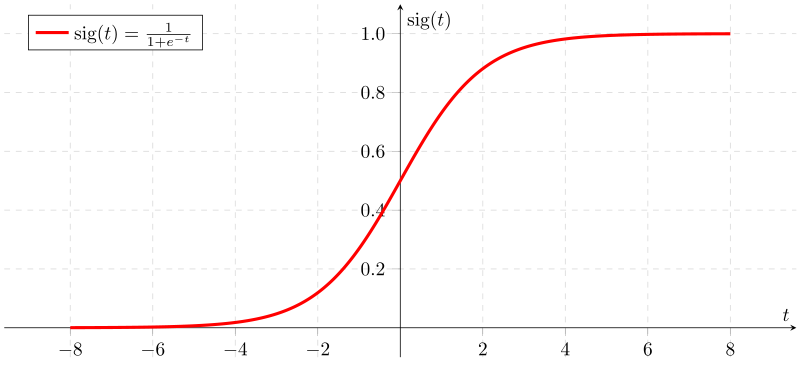
\includegraphics[width=0.8\textwidth]{img/Sigmoid-function-2.svg.png}
    \caption{Funzione sigmoidea. Immagine Tratta da \cite{Sigmoid_Function_Image}}
    \label{fig:esempio}
\end{figure}

\newpage
\section{Conclusioni}
\section{Conclusioni}
In questo capitolo sono stati introdotti i concetti fondamentali del \textit{Machine Learning}, analizzando i principali paradigmi di apprendimento (supervisionato, non supervisionato e per rinforzo), l’importanza dei dati e delle loro proprietà statistiche, le problematiche più comuni e i metodi di valutazione delle prestazioni dei modelli.
Inoltre, è stato presentato il modello della regressione logistica, utile per comprendere la struttura e il funzionamento delle reti neurali. Queste nozioni rappresentano le basi teoriche necessarie per affrontare i capitoli successivi, dedicati alla modellazione tramite reti neurali, che approfondiscono concetti già introdotti come le funzioni di loss, l’ottimizzazione e la capacità di generalizzazione.

\chapter{Reti Neurali}

\section{Introduzione}
\begin{flushleft}
In questo capitolo ci addentreremo nello studio delle reti neurali, iniziando dall'elemento più semplice, il \textbf{percettrone}, e proseguendo verso la costruzione di reti più complesse.
Verranno approfonditi concetti già introdotti nel Capitolo~1, come le funzioni di attivazione, essenziali per introdurre non linearità nei modelli, e i metodi basati sul gradiente per l'ottimizzazione dei parametri, compresa l'inizializzazione dei pesi e altre tecniche fondamentali per garantire un apprendimento efficace. 

Questa trattazione fornirà le basi teoriche necessarie per comprendere pienamente i capitoli successivi, in cui verrà presentata la rete MLP impiegata negli esperimenti di questa tesi. 
\end{flushleft}

\section{Concetti Fondamentali delle Reti Neurali}
\begin{flushleft}
    Le reti neurali artificiali costituiscono una classe di modelli computazionali ispirati al funzionamento dei sistemi nervosi biologici. Sebbene rappresentino una notevole semplificazione rispetto alla complessità delle reti neurali naturali, esse si dimostrano efficaci nella risoluzione di problemi complessi di intelligenza artificiale, dalla classificazione automatica di dati al riconoscimento di pattern sofisticati.

    L'unità computazionale fondamentale è il \textbf{percettrone}, il quale riceve molteplici segnali di input, li elabora attraverso funzioni di attivazione non lineari e genera un output. La comunicazione tra neuroni avviene mediante collegamenti pesati, denominati pesi sinaptici, che memorizzano informazioni apprese e determinano l'intensità dell'influenza che un neurone esercita sui successivi. Questa architettura integra strettamente memoria e capacità di calcolo, consentendo alla rete di apprendere automaticamente dai dati e di adattarsi dinamicamente a nuovi input.
    
    Una caratteristica distintiva delle reti neurali è il parallelismo computazionale: numerosi neuroni elaborano simultaneamente i segnali, creando un sistema distribuito di processori elementari ma coordinati. Questo approccio permette di affrontare problemi di elevata complessità senza la necessità di programmare esplicitamente ogni aspetto della soluzione, sfruttando invece la capacità emergente della rete di identificare pattern e relazioni nei dati.
    
    Storicamente, i primi modelli risalgono a McCulloch e Pitts (1943) con il neurone binario, seguiti dalle prime idee di apprendimento di Hebb (1949). Il perceptrone di Rosenblatt (1958) introdusse pesi variabili, rendendo possibile l'apprendimento, ma la sua limitata capacità portò a un periodo di stagnazione della ricerca fino agli anni '80. La generalizzazione ai problemi non linearmente separabili fu resa possibile dall'algoritmo di retropropagazione (BP) sviluppato da Rumelhart, Hinton e Williams (1986), che utilizza la discesa del gradiente per aggiornare i pesi in funzione dell'errore tra output desiderato e output effettivo.
    Oggi, le reti neurali a più livelli (MLP) addestrate con BP sono largamente impiegate in applicazioni di visione artificiale, elaborazione del linguaggio e sistemi intelligenti, grazie alla loro capacità di generalizzare da esempi e affrontare compiti complessi.
\end{flushleft}

\section{Il percettrone}
\begin{flushleft}
Il percettrone è l'elemento base di processo delle reti neurali artificiali e rappresenta il fondamento teorico su cui si basano i moderni sistemi di machine learning. Proposto per la prima volta da Frank Rosenblatt nel 1957, questo modello matematico è ispirato al funzionamento dei neuroni biologici e costituisce la più semplice forma di neurone artificiale.

\newpage
\subsection{Struttura e Funzionamento}
Il percettrone ha molti input, che possono essere forniti dall'ambiente o essere output di altri percettroni. Associato ad ogni input $x_{j} \in \mathbb{R},j = 1,....,d$, c'è un valore chiamato peso sinaptico $w_{j} \in \mathbb{R}$, e l'output $y$, nel caso più semplice è una somma pesata degli input:
\[
 \hspace{0.5cm} y=\sum_{j=1}^{d} w_j x_j + w_0
\]
Il termine $w_0$ è l'intercetta (o bias) che rende il modello più generale, ed è generalmente modellato come un peso proveniente da un'unità di bias extra,$x_0$, la quale assume sempre il valore $+1$.

\begin{figure}[h!]
\centering
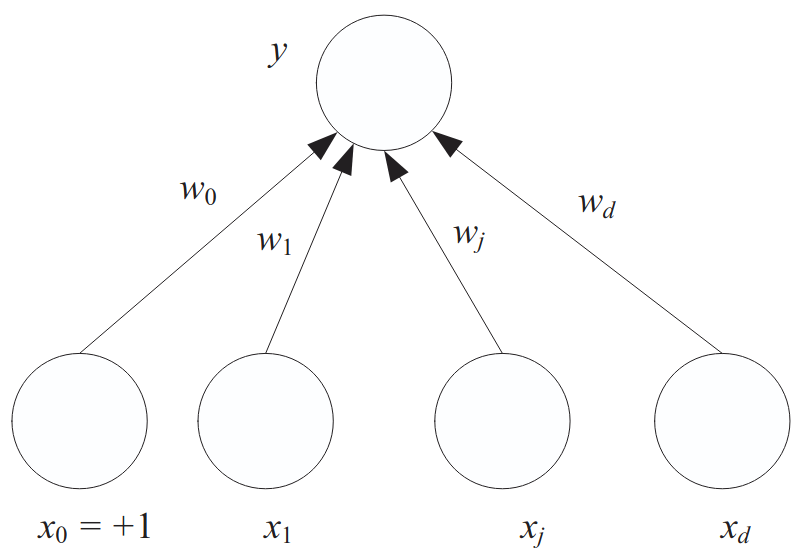
\includegraphics[width=0.4\textwidth]{img/single_perceptron.png}
\caption{Singolo percettrone.  Immagine tratta da \cite{Introduction_to_Machine_Learning_book}}
\label{fig:singolo percettrone}
\end{figure}

\subsection{Funzione di Attivazione}
Nella sua formulazione classica, il percettrone utilizza una funzione di attivazione a soglia (step function) per produrre l'output finale:
\[
\hat{y} = \begin{cases} 
1 & \text{se } y \geq \theta \\
0 & \text{se } y < \theta
\end{cases}
\]
dove $\theta$ è la soglia di attivazione. Questa funzione determina se il neurone si attiva o meno in base al valore della combinazione lineare degli input.

\newpage
\subsection{Interpretazione Geometrica}
Dal punto di vista geometrico, il percettrone definisce un iperpiano nello spazio degli input. L'equazione $\sum_{j=1}^{d} w_j x_j + w_0 = 0$ rappresenta infatti un iperpiano di dimensione $d-1$ in uno spazio $d$-dimensionale. I pesi $w_j$ determinano l'orientamento dell'iperpiano, mentre il bias $w_0$ ne determina la posizione. Il percettrone classifica i punti dello spazio assegnandoli a una delle due classi in base a quale lato dell'iperpiano si trovano.

\subsection{Limitazioni del Percettrone Singolo}
Il percettrone singolo presenta alcune limitazioni fondamentali:
\begin{itemize}
\item \textbf{Linearità}: Può risolvere solo problemi linearmente separabili, ovvero quelli in cui le classi possono essere separate da un iperpiano lineare.
\item \textbf{Funzioni non rappresentabili}: Non può rappresentare funzioni logiche semplici come XOR, che richiedono una separazione non lineare.
\item \textbf{Capacità espressiva limitata}: La sua capacità di apprendimento è limitata a pattern lineari nei dati.
\end{itemize}


\subsection{Algoritmo di Apprendimento}
L'algoritmo di apprendimento del percettrone è un processo iterativo che aggiorna i pesi in base agli errori di classificazione:
\begin{enumerate}
\item Inizializzare i pesi con valori casuali piccoli
\item Per ogni esempio di training $(x^{(i)}, t^{(i)})$:
\begin{itemize}
\item Calcolare l'output $\hat{y}^{(i)}$
\item Se $\hat{y}^{(i)} \neq t^{(i)}$, aggiornare i pesi:
\[w_j := w_j + \eta (t^{(i)} - \hat{y}^{(i)}) x_j^{(i)}\]
dove $\eta$ è il tasso di apprendimento (learning rate)
\end{itemize}
\end{enumerate}

Nonostante le sue limitazioni, il percettrone ha avuto un impatto fondamentale nello sviluppo delle reti neurali artificiali. La comprensione delle sue proprietà e limitazioni ha portato allo sviluppo del percettrone multi-strato (Multi-Layer Perceptron, MLP) e degli algoritmi di backpropagation, che costituiscono la base delle moderne deep neural networks. Il percettrone rimane un modello di riferimento importante per comprendere i principi fondamentali dell'apprendimento automatico e viene ancora utilizzato in applicazioni dove la semplicità e l'interpretabilità sono prioritarie rispetto alla complessità del modello.
\end{flushleft}

\section{Multi-Layer Perceptron}
\begin{flushleft}
Il Multi-Layer Perceptron (MLP) rappresenta l'evoluzione naturale del percettrone singolo per superarne le limitazioni fondamentali. Mentre il percettrone classico può risolvere solo problemi linearmente separabili, l'MLP introduce uno o più livelli nascosti (hidden layers) che conferiscono alla rete la capacità di apprendere relazioni non lineari complesse nei dati.

\subsection{Architettura}
Un MLP è composto da almeno tre tipi di livelli:
\begin{itemize}
\item \textbf{Livello di input}: Riceve i dati dall'ambiente esterno
\item \textbf{Livelli nascosti}: Uno o più livelli intermedi che processano le informazioni
\item \textbf{Livello di output}: Produce la risposta finale della rete
\end{itemize}

Ogni neurone in un livello è completamente connesso a tutti i neuroni del livello successivo, da cui il termine "fully connected" o "dense layer". Per un livello $l$ con $n^{(l)}$ neuroni, l'output del neurone $i$ è dato da:
\[
z_i^{(l)} = \sum_{j=1}^{n^{(l-1)}} w_{ij}^{(l)} a_j^{(l-1)} + b_i^{(l)}
\]
\[
a_i^{(l)} = f(z_i^{(l)})
\]
dove $w_{ij}^{(l)}$ sono i pesi, $b_i^{(l)}$ sono i bias, $a_j^{(l-1)}$ sono le attivazioni del livello precedente e $f(\cdot)$ è la funzione di attivazione.


\begin{figure}[h!]
    \centering
    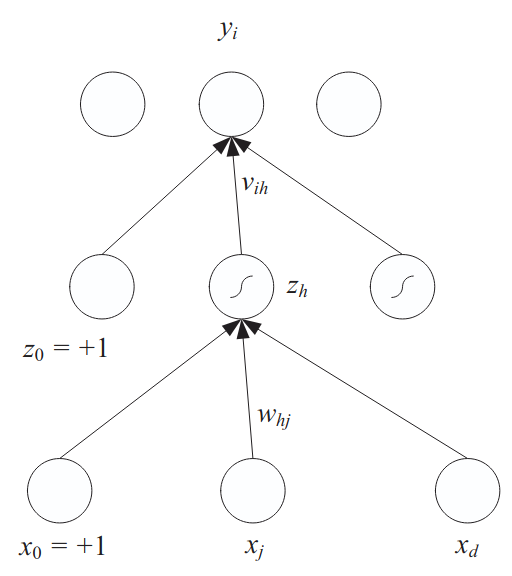
\includegraphics[width=0.4\textwidth]{img/Multi-Layer-Perceptron.png}
    \caption{Architettura Multi Layer Perceptrom. Immagine tratta da \cite{Introduction_to_Machine_Learning_book}}
    \label{fig: Architettura Multi Layer Perceptrom}
\end{figure}
    
\newpage
\subsection{Funzioni di Attivazione Non Lineari}
A differenza del percettrone classico che utilizza una funzione d'attivazione a soglia, l'MLP impiega funzioni di attivazione non lineari e differenziabili, essenziali per l'apprendimento tramite backpropagation. Le più comuni includono:
\begin{itemize}
\item \textbf{Sigmoide}: $f(x) = \frac{1}{1 + e^{-x}}$
\item \textbf{Tanh}: $f(x) = \frac{e^x - e^{-x}}{e^x + e^{-x}}$
\item \textbf{ReLU}: $f(x) = \max(0, x)$
\end{itemize}

\subsection{Funzione Softmax per Classificazione Multi-classe}
Nel livello di output per problemi di classificazione multi-classe, viene spesso utilizzata la funzione softmax, che trasforma un vettore di valori reali in una distribuzione di probabilità:
\[
\text{softmax}(z_i) = \frac{e^{z_i}}{\sum_{j=1}^K e^{z_j}}
\]
dove $z_i$ è l'input del neurone $i$ e $K$ è il numero totale di classi.

Le proprietà fondamentali della softmax sono:
\begin{itemize}
\item \textbf{Normalizzazione}: $\sum_{i=1}^K \text{softmax}(z_i) = 1$
\item \textbf{Monotonicità}: Preserva l'ordinamento relativo degli input
\item \textbf{Differenziabilità}: Essenziale per il calcolo dei gradienti
\end{itemize}

La softmax è particolarmente efficace quando combinata con la cross-entropy loss, formando una coppia matematicamente elegante per l'ottimizzazione. A differenza della funzione sigmoide, che è utilizzata per classificazione binaria, la softmax estende naturalmente il concetto a problemi multi-classe, garantendo che l'output rappresenti una distribuzione di probabilità valida su tutte le possibili classi.


\subsection{Teorema di Approssimazione Universale}
Un risultato teorico fondamentale stabilisce che un MLP con un singolo livello nascosto di dimensione sufficientemente grande può approssimare qualsiasi funzione continua con precisione arbitraria. Questo teorema, dimostrato da Cybenko (1989) e Hornik (1991), fornisce la base teorica per la capacità espressiva delle reti neurali.

\end{flushleft}

\section{Backpropagation}
\begin{flushleft}
L'algoritmo di backpropagation, sviluppato da Rumelhart, Hinton e Williams nel 1986, risolve il problema fondamentale di come addestrare reti neurali multi-strato. L'idea centrale consiste nel calcolare il gradiente della funzione di costo rispetto ai pesi della rete propagando l'errore all'indietro attraverso i livelli.


\subsection{Derivazione Matematica}
Consideriamo una funzione di costo $J(\theta)$ dove $\theta$ rappresenta tutti i parametri della rete. L'obiettivo è minimizzare $J$ aggiornando i pesi secondo la regola:
\[
w_{ij}^{(l)} := w_{ij}^{(l)} - \eta \frac{\partial J}{\partial w_{ij}^{(l)}}
\]

Utilizzando la regola della catena, il gradiente può essere scomposto come:
\[
\frac{\partial J}{\partial w_{ij}^{(l)}} = \frac{\partial J}{\partial z_i^{(l)}} \frac{\partial z_i^{(l)}}{\partial w_{ij}^{(l)}} = \delta_i^{(l)} a_j^{(l-1)}
\]

dove $\delta_i^{(l)} = \frac{\partial J}{\partial z_i^{(l)}}$ è l'errore del neurone $i$ nel livello $l$.

Per il livello di output:
\[
\delta_i^{(L)} = \frac{\partial J}{\partial a_i^{(L)}} f'(z_i^{(L)})
\]

Per i livelli nascosti, l'errore si propaga all'indietro:
\[
\delta_i^{(l)} = \left(\sum_{k=1}^{n^{(l+1)}} w_{ki}^{(l+1)} \delta_k^{(l+1)}\right) f'(z_i^{(l)})
\]

\subsection{Algoritmo di Gradient Descent}
Il gradient descent è l'algoritmo di ottimizzazione fondamentale utilizzato con backpropagation, e ha la seguente struttura:

\begin{enumerate}
\item \textbf{Forward pass}: Calcola le attivazioni per tutti i livelli
\item \textbf{Calcolo del costo}: Valuta la funzione di costo sull'output
\item \textbf{Backward pass}: Calcola i gradienti propagando l'errore all'indietro
\item \textbf{Aggiornamento parametri}: $\theta := \theta - \eta \nabla_\theta J$
\end{enumerate}

Le varianti principali includono:
\begin{itemize}
\item \textbf{Batch Gradient Descent}: Utilizza l'intero dataset per ogni aggiornamento
\item \textbf{Stochastic Gradient Descent (SGD)}: Aggiorna i pesi utilizzando un singolo esempio
\item \textbf{Mini-batch Gradient Descent}: Compromesso che utilizza piccoli batch di dati
\end{itemize}

\subsection{Algoritmo Adam}
Adam (Adaptive Moment Estimation) è un algoritmo di ottimizzazione avanzato che combina i vantaggi di AdaGrad e RMSprop. Mantiene medie mobili esponenziali sia del gradiente che del suo quadrato:

\begin{align}
m_t &= \beta_1 m_{t-1} + (1 - \beta_1) g_t \\
v_t &= \beta_2 v_{t-1} + (1 - \beta_2) g_t^2 \\
\hat{m}_t &= \frac{m_t}{1 - \beta_1^t} \\
\hat{v}_t &= \frac{v_t}{1 - \beta_2^t} \\
\theta_t &= \theta_{t-1} - \frac{\eta}{\sqrt{\hat{v}_t} + \epsilon} \hat{m}_t
\end{align}

dove $g_t$ è il gradiente al tempo $t$, $\beta_1$ e $\beta_2$ sono i fattori di decadimento (tipicamente 0.9 e 0.999), ed $\epsilon$ è una piccola costante per la stabilità numerica.


\subsection{Problema dei Minimi Locali}
I metodi basati sul gradiente presentano diverse sfide teoriche e pratiche:

\begin{itemize}
\item \textbf{Minimi locali}: La funzione di costo può avere molteplici minimi locali dove il gradiente è zero, ma che non rappresentano la soluzione ottimale globale.

\item \textbf{Punti di sella}: In dimensioni elevate, la maggior parte dei punti critici sono punti di sella piuttosto che minimi locali, dove alcune direzioni sono discendenti e altre ascendenti.

\item \textbf{Plateau}: Regioni quasi piatte della superficie di costo dove il gradiente è molto piccolo, causando convergenza lenta.

\item \textbf{Vanishing gradients}: Nei livelli più profondi, i gradienti possono diventare estremamente piccoli, rendendo l'apprendimento inefficace.

\item \textbf{Exploding gradients}: Ib questo caso i gradienti possono crescere esponenzialmente, causando instabilità numerica.
\end{itemize}

Moderne tecniche di regolarizzazione, architetture migliorate e algoritmi di ottimizzazione adattivi aiutano a mitigare questi problemi, rendendo l'addestramento di reti profonde più stabile ed efficace.

\end{flushleft}

\section{Inizializzazione dei Pesi}
\begin{flushleft}
L'inizializzazione dei pesi rappresenta un aspetto critico nell'addestramento delle reti neurali che può determinare il successo o il fallimento del processo di apprendimento. Una cattiva inizializzazione può portare a problemi di vanishing o exploding gradients, convergenza lenta o blocco in minimi locali sfavorevoli.

\subsection{Problematiche dell'Inizializzazione Casuale}
L'inizializzazione naive con valori casuali uniformi o gaussiani può causare diversi problemi:
\begin{itemize}
\item \textbf{Saturazione delle attivazioni}: Valori troppo grandi possono saturare le funzioni di attivazione (es. sigmoide), causando gradienti quasi nulli
\item \textbf{Simmetria}: Inizializzare tutti i pesi con lo stesso valore porta alla perdita della capacità di apprendimento
\item \textbf{Scaling inadeguato}: La varianza delle attivazioni può crescere o diminuire drasticamente attraverso i livelli
\end{itemize}

\subsection{Inizializzazione Xavier/Glorot}
Proposta da Glorot e Bengio (2010), questa tecnica mira a mantenere la varianza delle attivazioni costante attraverso tutti i livelli. Per un livello con $n_{in}$ input e $n_{out}$ output, i pesi sono inizializzati con:

\textbf{Distribuzione uniforme}:
\[
w \sim U\left(-\sqrt{\frac{6}{n_{in} + n_{out}}}, \sqrt{\frac{6}{n_{in} + n_{out}}}\right)
\]

\textbf{Distribuzione normale}:
\[
w \sim \mathcal{N}\left(0, \sqrt{\frac{2}{n_{in} + n_{out}}}\right)
\]

Questa inizializzazione è ottimale per funzioni di attivazione lineari e tanh, mantenendo la varianza delle attivazioni approssimativamente costante durante il forward pass.


\subsection{Inizializzazione He}
Sviluppata da He et al. (2015), questa tecnica è specificamente progettata per funzioni ReLU e loro varianti. Considerando che ReLU azzera metà degli input, la varianza deve essere compensata di conseguenza:

\[
w \sim \mathcal{N}\left(0, \sqrt{\frac{2}{n_{in}}}\right)
\]

Questa inizializzazione tiene conto del fatto che ReLU elimina i valori negativi, mantenendo così una varianza appropriata nel signal propagation.

\subsection{Altre Tecniche di Inizializzazione}
\begin{itemize}
\item \textbf{LeCun initialization}: $w \sim \mathcal{N}(0, \sqrt{1/n_{in}})$, adatta per funzioni SELU
\item \textbf{LSUV (Layer-wise Sequential Unit-Variance)}: Inizializzazione iterativa che normalizza la varianza layer per layer
\end{itemize}

\subsection{Impatto Pratico}
Una corretta inizializzazione può ridurre significativamente il tempo di addestramento e migliorare le prestazioni finali del modello. La scelta del metodo dipende dall'architettura della rete, dalle funzioni di attivazione utilizzate e dalla profondità del modello. Nelle reti moderne, l'inizializzazione He è diventata lo standard per architetture basate su ReLU, mentre Xavier rimane preferita per reti con attivazioni sigmoidi o tanh.

L'importanza dell'inizializzazione è stata ulteriormente evidenziata con lo sviluppo di reti sempre più profonde, dove piccole variazioni nell'inizializzazione possono avere effetti amplificati attraverso molti livelli, influenzando di molto la capacità della rete di apprendere rappresentazioni significative.

\end{flushleft}

\section{Overparametrizzazione delle Reti Neurali}
\begin{flushleft}
L'overparametrizzazione rappresenta uno dei fenomeni più controintuitivi del machine learning moderno, dove le reti neurali sono progettate per avere più parametri di quelli strettamente necessari per rappresentare la funzione target. Questo concetto sfida la saggezza convenzionale del bias-variance trade-off e ha rivoluzionato la comprensione di come le reti neurali apprendono e generalizzano.

\subsection{Il Paradosso della Generalizzazione}
Tradizionalmente, il bias-variance trade-off suggeriva che modelli troppo complessi cadrebbero inevitabilmente in overfitting. Tuttavia, nella pratica moderna, reti neurali con milioni di parametri che interpolano perfettamente i dati di training spesso mostrano eccellenti prestazioni di generalizzazione. Questo fenomeno, noto come \textit{benign overfitting}, indica che nelle reti overparametrizzate il trade-off classico si manifesta in modo diverso: il bias rimane basso mentre la varianza viene controllata attraverso meccanismi di regolarizzazione implicita.

\begin{figure}[h!]
    \centering
    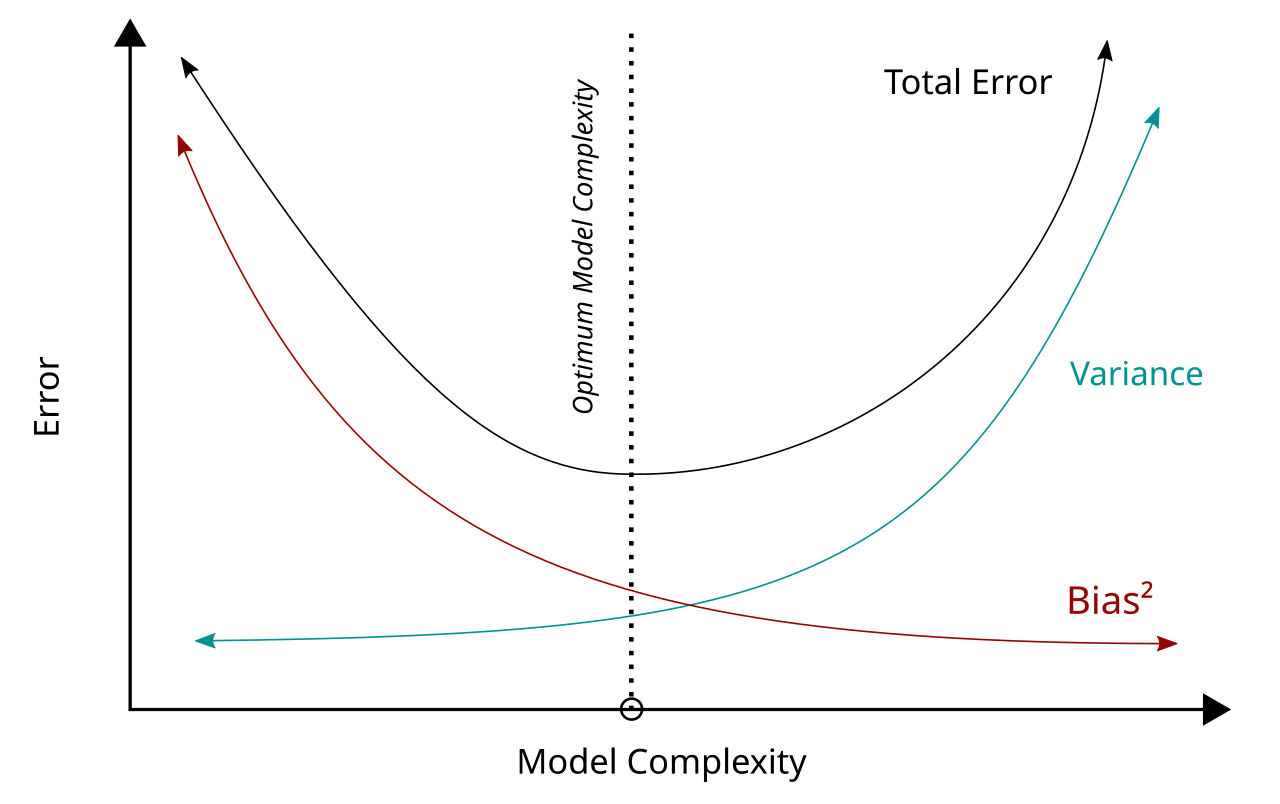
\includegraphics[width=0.6\textwidth]{img/Bias_and_variance_contributing_to_total_error.svg.png}
    \caption{Bias–variance tradeoff. Immagine tratta da \cite{Bias_Variance_Image}}
    \label{fig:Bias–variance tradeoff}
\end{figure}
    
\newpage
\subsection{Il Fenomeno del Double Descent}
Il fenomeno del double descent descrive una curva di rischio che presenta tre regioni distinte:
\begin{enumerate}
\item \textbf{Regime underparameterizzato}: Comportamento classico dove aumentare la complessità migliora le prestazioni fino a un optimum
\item \textbf{Regime critico}: Zona di interpolazione dove il modello fitta perfettamente i dati di training ($\text{Training error} = 0$), spesso con prestazioni di test scadenti
\item \textbf{Regime overparameterizzato}: Oltre la soglia di interpolazione, ulteriori aumenti dei parametri migliorano nuovamente le prestazioni di test
\end{enumerate}

\begin{figure}[h!]
    \centering
    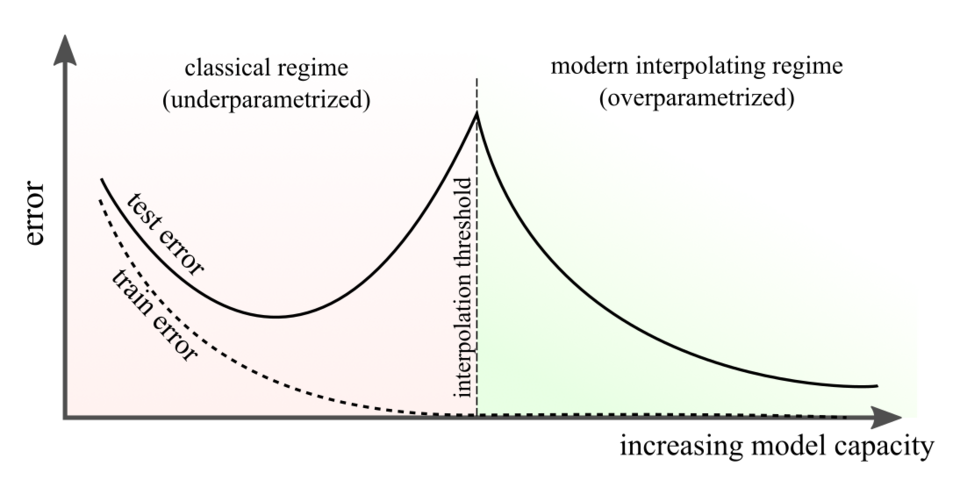
\includegraphics[width=0.7\textwidth]{img/Double_descent.png}
    \caption{Double Descent. Immagine tratta da \cite{Double_Descent_Image}}
    \label{fig:Double Descent}
\end{figure}

\subsection{Differenze tra Reti Piccole e Grandi}
Le dinamiche di apprendimento cambiano drasticamente tra reti di diverse dimensioni:

\subsubsection{Reti Piccole (Underparameterizzate)}
Nelle reti con pochi parametri rispetto alla complessità del problema:
\begin{itemize}
\item \textbf{Sensibilità all'inizializzazione}: La scelta dell'inizializzazione diventa critica poiché lo spazio dei parametri è limitato
\item \textbf{Minimi locali problematici}: Maggior rischio di rimanere bloccati in minimi locali subottimali
\item \textbf{Metodi di ricerca cruciali}: L'algoritmo di ottimizzazione (SGD vs Adam) può fare la differenza tra convergenza e fallimento
\item \textbf{Capacità limitata}: Impossibilità di catturare pattern complessi nei dati
\end{itemize}

\subsubsection{Reti Grandi (Overparameterizzate)}
Nelle reti con molti parametri:
\begin{itemize}
\item \textbf{Robustezza all'inizializzazione}: Meno sensibili alla scelta iniziale dei pesi
\item \textbf{Landscape più favorevole}: Presenza di numerosi minimi locali di qualità simile, spesso connessi attraverso percorsi di bassa perdita
\item \textbf{Regolarizzazione implicita}: Meccanismi intrinseci che prevengono l'overfitting, inclusi il bias induttivo di SGD verso soluzioni con margine ampio e l'effetto regolarizzante del rumore nel gradiente
\item \textbf{Lottery ticket hypothesis}: Esistenza di sotto-reti sparse che mantengono le prestazioni
\end{itemize}

\subsection{Importanza del Metodo di Ricerca}
Nelle reti piccole, il metodo di ottimizzazione assume un ruolo fondamentale: il gradient descent classico può facilmente rimanere intrappolato in minimi locali, mentre algoritmi adattivi come Adam possono aiutare l'esplorazione dello spazio dei parametri. La scelta del learning rate, dello scheduler e della strategia di momentum diventa critica quando i gradi di libertà sono limitati.

Al contrario, nelle reti grandi, diversi algoritmi di ottimizzazione tendono a convergere a soluzioni con prestazioni simili, suggerendo che il landscape di ottimizzazione è intrinsecamente più favorevole. 

L'overparametrizzazione facilita l'ottimizzazione anche per metodi non gradient-based, come gli algoritmi evolutivi, poiché aumenta il numero di configurazioni di parametri che portano a soluzioni accettabili, rendendo lo spazio di ricerca più 'denso' di buone soluzioni.
\end{flushleft}

\section{Conclusioni}
\begin{flushleft}
In questo capitolo sono stati presentati i concetti fondamentali delle reti neurali, che serviranno a comprendere completamente quello che sarà successivamente trattato. Dal percettrone singolo ai Multi-Layer Perceptron, dall'algoritmo di backpropagation alle tecniche di inizializzazione, fino al paradosso dell'overparametrizzazione, questi elementi costituiscono la base teorica e pratica necessaria per affrontare architetture più avanzate e applicazioni specifiche che saranno discusse nei capitoli successivi.
\end{flushleft}
\chapter{Algortimi Genetici}

\section{Algoritmi Evolutivi}
\begin{flushleft}
Gli algoritmi evolutivi rappresentano una classe di metodi di ottimizzazione che si basano sui principi fondamentali della teoria dell'evoluzione darwiniana, in particolare sul concetto di selezione naturale e sopravvivenza del più adatto. Questi algoritmi operano mantenendo una popolazione di soluzioni candidate che evolve iterativamente attraverso operatori che mimano i processi biologici di riproduzione, mutazione e selezione.

Il paradigma evolutivo si articola attorno a alcuni concetti chiave: una \textbf{popolazione} costituita da individui che rappresentano potenziali soluzioni al problema di ottimizzazione, una \textbf{funzione di fitness} che valuta quantitativamente la qualità di ciascuna soluzione, e un insieme di \textbf{operatori evolutivi} che generano nuove soluzioni a partire da quelle esistenti. Il processo iterativo, denominato \textbf{generazione}, applica ripetutamente questi operatori fino al raggiungimento di un criterio di convergenza.

La forza degli algoritmi evolutivi risiede nella loro capacità di esplorare efficacemente spazi di ricerca complessi e multimodali. Questa caratteristica li rende particolarmente adatti per problemi di ottimizzazione discontinui, non differenziabili o caratterizzati da rumore.

Gli algoritmi evolutivi comprendono diverse sottocategorie, ciascuna con caratteristiche e domini applicativi specifici:
\begin{itemize}
\item \textbf{Algoritmi Genetici (GA)}: Operano su rappresentazioni binarie o reali delle soluzioni, utilizzando crossover e mutazione come operatori principali
\item \textbf{Genetic Programming (GP)}: Evolve programmi o espressioni matematiche rappresentate come alberi sintattici
\item \textbf{Evolution Strategies (ES)}: Focalizzati sull'ottimizzazione di parametri reali con particolare attenzione all'auto-adattamento
\end{itemize}

La versatilità e la robustezza di questi approcci hanno portato al loro ampio utilizzo in svariati domini applicativi, dall'ottimizzazione di parametri nell'ingegneria alla progettazione automatica di circuiti, dall'addestramento di reti neurali alla risoluzione di problemi combinatoriali complessi.
\end{flushleft}


\section{Algoritmi Genetici}
\begin{flushleft}
Gli Algoritmi Genetici (GA), introdotti da John Holland negli anni '70, rappresentano la forma più classica e studiata degli algoritmi evolutivi. Questi algoritmi operano su una popolazione di cromosomi, ciascuno dei quali codifica una potenziale soluzione al problema di ottimizzazione. Il processo evolutivo avviene attraverso l'applicazione iterativa di operatori genetici che mimano i meccanismi biologici fondamentali.

\subsection{Rappresentazione e Codifica}
La rappresentazione delle soluzioni costituisce un aspetto fondamentale nella progettazione di un algoritmo genetico. Le codifiche più comuni includono:
\begin{itemize}
\item \textbf{Codifica binaria}: Ogni gene è rappresentato da un bit (0 o 1)
\item \textbf{Codifica reale}: I geni assumono valori in numeri reali
\item \textbf{Codifica ad albero}: Impiegata quando le soluzioni hanno struttura gerarchica
\end{itemize}

\subsection{Operatori Genetici Fondamentali}

\subsubsection{Selezione}
La selezione determina quali individui della popolazione corrente avranno la possibilità di riprodursi e contribuire alla generazione successiva. I metodi principali includono:

\begin{itemize}
    \item \textbf{Selezione proporzionale (Roulette Wheel):} La probabilità di selezione è proporzionale alla fitness dell'individuo:
    \[
    P_i = \frac{f_i}{\sum_{j=1}^{N} f_j}
    \]
    dove $f_i$ è la fitness dell'individuo $i$ e $N$ è la dimensione della popolazione.
    
    \item \textbf{Selezione a torneo:} Un sottoinsieme casuale di individui compete, e il migliore viene selezionato. La pressione selettiva può essere controllata variando la dimensione del torneo.
    
    \item \textbf{Selezione per ranking:} Gli individui sono ordinati per fitness e la selezione avviene in base alla posizione nella classifica piuttosto che al valore assoluto di fitness.
\end{itemize}

\subsubsection{Crossover}
Il crossover combina materiale genetico di due o più genitori per produrre la prole. Per la codifica binaria, i metodi classici includono:
\begin{itemize}
    \item \textbf{Crossover a punto singolo:} Un punto di taglio divide i cromosomi, e i segmenti vengono scambiati tra i genitori.

    \item \textbf{Crossover a punti multipli:} Utilizza più punti di taglio, alternando i segmenti tra i genitori.

    \item \textbf{Crossover uniforme:} Ogni gene della prole è scelto casualmente da uno dei due genitori con probabilità fissa.
\end{itemize}

\subsubsection{Mutazione}
La mutazione introduce variabilità nella popolazione modificando casualmente alcuni geni degli individui. Serve a:
\begin{itemize}
\item Mantenere la diversità genetica nella popolazione
\item Esplorare nuove regioni dello spazio di ricerca
\item Prevenire la convergenza prematura
\end{itemize}

Per la codifica binaria, la mutazione tipicamente inverte bit casuali con una probabilità di mutazione $p_m$ generalmente bassa (0.001-0.01). Per la codifica reale, si applicano perturbazioni gaussiane:
\[
x'_i = x_i + \mathcal{N}(0, \sigma^2)
\]

\subsubsection{Elitismo}
L'elitismo garantisce che i migliori individui di una generazione sopravvivano alla successiva, preservando le soluzioni di alta qualità già trovate. Questo meccanismo:
\begin{itemize}
\item Accelera la convergenza dell'algoritmo
\item Previene la perdita di soluzioni ottime già scoperte
\item Può essere implementato preservando una percentuale fissa dei migliori individui
\end{itemize}

\begin{figure}[h!]
    \centering
    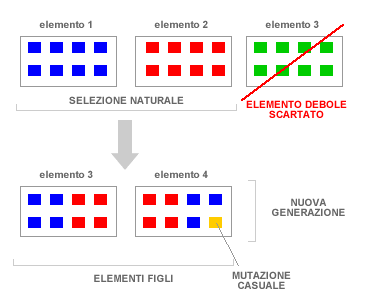
\includegraphics[width=0.5\textwidth]{img/algoritmo-genetico-schema.png}
    \caption{Schema Algortitmi Genetici. Immagine tratta da \cite{GA_Image}}
    \label{fig:Schema Algotmi Genetici}
\end{figure}

\subsection{Schema dell'Algoritmo Genetico}
Il ciclo evolutivo standard segue questi passaggi:
\begin{enumerate}
\item \textbf{Inizializzazione}: Genera una popolazione iniziale casuale
\item \textbf{Valutazione}: Calcola la fitness di ogni individuo
\item \textbf{Controllo terminazione}: Verifica i criteri di stop
\item \textbf{Selezione}: Sceglie i genitori per la riproduzione
\item \textbf{Crossover}: Applica ricombinazione con probabilità $p_c$
\item \textbf{Mutazione}: Applica mutazione con probabilità $p_m$
\item \textbf{Rimpiazzamento}: Determina la nuova popolazione
\item \textbf{Ritorna al passo 2}
\end{enumerate}

\subsection{Parametri e Tuning}
Il successo di un algoritmo genetico dipende criticamente dalla scelta dei parametri:
\begin{itemize}
\item \textbf{Dimensione popolazione}: Tipicamente 50-500 individui
\item \textbf{Probabilità di crossover}: Generalmente alta (0.6-0.9)
\item \textbf{Probabilità di mutazione}: Generalmente bassa (0.001-0.1)
\end{itemize}

\end{flushleft}

\section{Metodi di Crossover per Codifica Reale}
\begin{flushleft}
Quando si lavora con problemi di ottimizzazione continua, la codifica reale richiede operatori di crossover specificamente progettati per preservare e ricombinare efficacemente l'informazione numerica. I metodi principali si distinguono per le loro proprietà matematiche e il comportamento esplorativo.


\subsection{Crossover Aritmetico}
Il crossover aritmetico genera la prole come combinazione lineare dei genitori:
\[
\begin{aligned}
\text{figlio}_1 &= \alpha \cdot \text{genitore}_1 + (1-\alpha) \cdot \text{genitore}_2 \\
\text{figlio}_2 &= (1-\alpha) \cdot \text{genitore}_1 + \alpha \cdot \text{genitore}_2
\end{aligned}
\]
dove $\alpha \in [0,1]$ è un parametro che controlla il peso della combinazione.

\textbf{Varianti principali:}
\begin{itemize}
\item \textbf{Uniforme}: $\alpha$ costante per tutti i geni
\item \textbf{Non-uniforme}: $\alpha$ varia per ogni gene
\item \textbf{Adattivo}: $\alpha$ cambia nel tempo o in base alla fitness
\end{itemize}

\textbf{Proprietà:} Garantisce che la prole rimanga nell'ipercubo definito dai genitori, assicurando exploiting delle regioni promettenti.

\subsection{Blend Crossover (BLX)}
Il Blend Crossover, proposto da Eshelman e Schaffer, estende l'intervallo di ricombinazione oltre i valori dei genitori. Per ogni gene $i$:
\[
\text{figlio}_i \sim U[x_{\min} - \alpha \cdot I, x_{\max} + \alpha \cdot I]
\]
dove:
\begin{itemize}
\item $x_{\min} = \min(\text{genitore}_{1,i}, \text{genitore}_{2,i})$
\item $x_{\max} = \max(\text{genitore}_{1,i}, \text{genitore}_{2,i})$
\item $I = x_{\max} - x_{\min}$
\item $\alpha$ controlla l'estensione dell'intervallo (tipicamente 0.5)
\end{itemize}

\textbf{Caratteristiche:}
\begin{itemize}
\item Bilancia exploration ed exploitation
\item Mantiene diversità nella popolazione
\item Può generare valori esterni all'intervallo parentale
\end{itemize}

\subsection{Simulated Binary Crossover (SBX)}
Il Simulated Binary Crossover, sviluppato da Deb e Agrawal, simula il comportamento del crossover a punto singolo per variabili continue. La distribuzione di probabilità della prole è definita da:
\[
P(x) = \frac{1}{2}(\eta + 1)(1 - |x - 0.5|)^\eta
\]
dove $\eta$ è l'indice di distribuzione che controlla la forma della distribuzione.

\textbf{Procedura SBX:}
\begin{enumerate}
\item Genera un numero casuale $u \sim U[0,1]$
\item Calcola il fattore di espansione:
\[
\beta = \begin{cases}
(2u)^{1/(\eta+1)} & \text{se } u \leq 0.5 \\
(1/(2(1-u)))^{1/(\eta+1)} & \text{se } u > 0.5
\end{cases}
\]
\item Genera la prole:
\[
\begin{aligned}
\text{figlio}_1 &= 0.5[(1+\beta)\text{genitore}_1 + (1-\beta)\text{genitore}_2] \\
\text{figlio}_2 &= 0.5[(1-\beta)\text{genitore}_1 + (1+\beta)\text{genitore}_2]
\end{aligned}
\]
\end{enumerate}

\textbf{Vantaggi di SBX:}
\begin{itemize}
\item Controllo preciso della dispersione tramite $\eta$
\item Comportamento auto-adattivo rispetto alla distanza parentale
\item Ampiamente utilizzato in algoritmi evolutivi multi-obiettivo
\item Preserva la media dei genitori
\end{itemize}

\subsection{Confronto e Scelta del Metodo}
La scelta del metodo di crossover dipende dalle caratteristiche del problema:
\begin{itemize}
\item \textbf{Crossover aritmetico}: Ideale per exploitation locale e convergenza rapida
\item \textbf{BLX}: Bilanciato per problemi che richiedono exploration moderata
\item \textbf{SBX}: Preferito per ottimizzazione multi-obiettivo e controllo fine della dispersione
\end{itemize}

\end{flushleft}

\section{Rappresentazione di Reti Neurali attraverso i GA}
\begin{flushleft}
La rappresentazione di reti neurali attraverso algoritmi genetici costituisce un approccio alternativo ai metodi di addestramento tradizionali basati sul gradiente. Questo paradigma consente di formulare l'ottimizzazione dei parametri di rete come un problema di ricerca evolutiva, aprendo nuove possibilità per l'esplorazione dello spazio dei pesi e superando alcune limitazioni intrinseche dei metodi gradient-based.

\subsection{Codifica dei Parametri di Rete}
Per applicare gli algoritmi genetici all'addestramento di reti neurali, è necessario definire una rappresentazione appropriata che mappi la struttura della rete in un cromosoma evolutivo. L'approccio più diretto e comunemente utilizzato consiste nella \textbf{codifica diretta dei pesi}, dove ogni individuo della popolazione è rappresentato come un vettore di valori reali:

\[
\mathbf{x} = [w_1, w_2, \ldots, w_n, b_1, b_2, \ldots, b_m]
\]

dove $w_i$ rappresentano i pesi sinaptici e $b_j$ i bias della rete. Questa rappresentazione concatena linearmente tutti i parametri della rete in un singolo cromosoma, mantenendo un ordine consistente che preservi la topologia delle connessioni.

\textbf{Vantaggi della codifica diretta:}
\begin{itemize}
\item Semplicità implementativa e concettuale
\item Applicabilità a qualsiasi architettura di rete
\item Compatibilità diretta con operatori genetici standard per valori reali
\end{itemize}

\textbf{Limitazioni:}
\begin{itemize}
\item Scalabilità limitata per reti di grandi dimensioni
\item Perdita di informazione strutturale nel cromosoma
\item Crescita quadratica dello spazio di ricerca rispetto alla dimensione della rete
\end{itemize}


\subsection{Funzione di Fitness}
La definizione della funzione di fitness rappresenta un elemento cruciale che determina la direzione dell'evoluzione. A differenza dei metodi gradient-based, gli algoritmi genetici permettono di utilizzare qualsiasi metrica valutabile, anche non differenziabile.
\subsubsection{Metriche Basate sulla Loss}
Le funzioni di loss tradizionali possono essere utilizzate direttamente come funzione di fitness negli algoritmi genetici. Non esiste una rappresentazione obbligatoria per la trasformazione loss-fitness; l'aspetto cruciale consiste nel definire correttamente se l'obiettivo è la minimizzazione o la massimizzazione della metrica scelta.

Gli approcci principali includono:
\begin{itemize}
\item \textbf{Utilizzo diretto}: Configurare l'algoritmo genetico per minimizzare la loss
\item \textbf{Negazione}: Utilizzare $\text{fitness} = -\text{loss}$ per massimizzazione
\item \textbf{Trasformazioni}: Applicare funzioni come $\text{fitness} = \frac{1}{1 + \text{loss}}$ per mappare in valori positivi
\end{itemize}

Le loss più comuni includono:
\begin{itemize}
\item \textbf{Mean Squared Error (MSE)}: $\text{MSE} = \frac{1}{N}\sum_{i=1}^{N}(y_i - \hat{y}_i)^2$
\item \textbf{Cross-Entropy}: $\text{CE} = -\frac{1}{N}\sum_{i=1}^{N}\sum_{c=1}^{C}y_{i,c}\log(\hat{y}_{i,c})$
\end{itemize}

\subsubsection{Metriche Alternative Non Differenziabili}
Una caratteristica distintiva degli algoritmi genetici è la possibilità di ottimizzare direttamente metriche di performance che non sono differenziabili, aprendo nuovi scenari di ottimizzazione:

\textbf{Accuracy:} La percentuale di predizioni corrette può essere utilizzata direttamente:
\[
\text{Accuracy} = \frac{1}{N}\sum_{i=1}^{N}\mathbb{I}[\arg\max(\hat{y}_i) = \arg\max(y_i)]
\]

\textbf{F1-Score:} Particolarmente utile per dataset sbilanciati:
\[
\text{F1} = \frac{2 \cdot \text{Precision} \cdot \text{Recall}}{\text{Precision} + \text{Recall}}
\]

\textbf{Metriche composite:} È possibile combinare multiple obiettivi:
\[
\text{fitness} = \alpha \cdot \text{Accuracy} + \beta \cdot \text{Complessità}^{-1} + \gamma \cdot \text{Robustezza}
\]


\subsection{Confronto con Metodi Gradient-Based}
L'utilizzo di algoritmi genetici per l'addestramento di reti neurali presenta caratteristiche distintive rispetto ai metodi tradizionali:

\textbf{Vantaggi degli algoritmi genetici:}
\begin{itemize}
\item \textbf{Robustezza ai minimi locali}: L'esplorazione population-based riduce il rischio di convergenza prematura
\item \textbf{Flessibilità nella funzione obiettivo}: Possibilità di ottimizzare metriche non differenziabili
\item \textbf{Parallelizzazione naturale}: La valutazione degli individui è intrinsecamente parallelizzabile
\item \textbf{Resistenza al rumore}: Meno sensibili a valutazioni fitness rumorose
\end{itemize}

\textbf{Limitazioni rispetto ai metodi gradient-based:}
\begin{itemize}
\item \textbf{Efficienza computazionale}: Richiedono tipicamente più valutazioni della funzione obiettivo
\item \textbf{Scalabilità}: Problematici per reti con milioni di parametri
\item \textbf{Convergenza}: Generalmente più lenti nella fase di fine-tuning locale
\end{itemize}

Questa dualità di approcci evidenzia come gli algoritmi genetici possano essere particolarmente vantaggiosi in scenari specifici, quali l'ottimizzazione di architetture di rete, l'addestramento in ambienti multi-obiettivo, o quando la funzione di loss presenta caratteristiche non favorevoli ai metodi basati sul gradiente.

\end{flushleft}

\section{Conclusioni}
\begin{flushleft}
In questo capitolo sono stati presentati gli algoritmi evolutivi in generale e gli algoritmi genetici nello specifico. Sono stati analizzati i passaggi e le componenti principali che li caratterizzano, dedicando particolare attenzione ai diversi operatori genetici e focalizzandosi approfonditamente sui vari metodi di crossover, che rappresentano uno degli elementi fondamentali dei GA.

È stata inoltre esaminata la modalità di codifica e addestramento delle reti neurali attraverso l'utilizzo degli algoritmi genetici, evidenziando come questo approccio alternativo possa superare alcune limitazioni dei metodi tradizionali basati sul gradiente. Questa introduzione teorica costituisce la base necessaria per comprendere pienamente i capitoli successivi, dove verrà definita l'architettura specifica della rete neurale utilizzata, la sua rappresentazione attraverso GA, i metodi di crossover e mutazione implementati, nonché ulteriori tecniche di ottimizzazione applicate.


\end{flushleft}
\chapter{Strumenti Utilizzati}

\section{Introduzione}
    In questo capitolo verranno introdotti gli strumenti utilizzati per affrontare la tesi, in particolare ci si concentrerà su: \texttt{MNIST}, \texttt{PyTorch} e \texttt{DEAP}.


\section{MNIST}
Il dataset MNIST (Modified National Institute of Standards and Technology) è uno dei dataset più noti e utilizzati nel campo del machine learning e del riconoscimento di immagini scritte a mano. Esso contiene immagini in scala di grigi di dimensione $28 \times 28$ pixel rappresentanti cifre da 0 a 9, quindi ogni immagine ha una singola componente di colore e può essere rappresentata come un tensore con shape $(1,28, 28)$.  
\\MNIST è composto da 60.000 immagini per il training e 10.000 immagini per il testing, ed è particolarmente utile per sperimentare algoritmi di classificazione perché le immagini sono già normalizzate e centrate. Ogni immagine è accompagnata da un’etichetta che indica quale cifra rappresenta (da 0 a 9), rendendo il dataset un tipico problema di classificazione supervisionata a 10 classi.  
\\Il dataset è stato originariamente derivato dal NIST, ma successivamente è stato preprocessato e ridimensionato da LeCun et al. per rendere le immagini più uniformi e facilmente utilizzabili dagli algoritmi di machine learning. La semplicità e la standardizzazione di MNIST lo rendono ideale per testare nuovi modelli, confrontare algoritmi di ottimizzazione e valutare rapidamente la capacità di una rete neurale di apprendere rappresentazioni visive.  
\begin{figure}[h!]
    \centering
    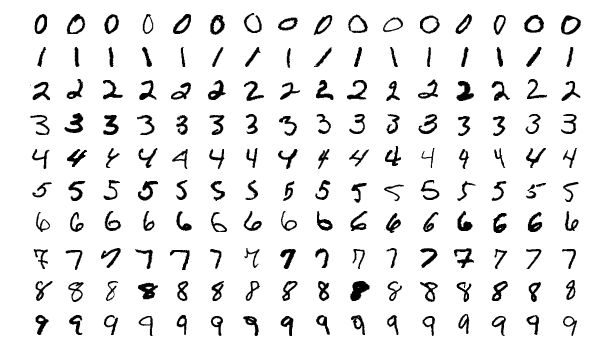
\includegraphics[width=0.5\textwidth]{img/MnistExamples.png}
    \caption{Dataset MNIST. Immagine tratta da \cite{MNIST_Examples_Image}}
    \label{fig:Dataset_MNIST}
\end{figure}

\section{PyTorch}

PyTorch è un framework open-source per il deep learning sviluppato dal laboratorio \textit{Facebook AI Research} (FAIR) e rilasciato per la prima volta nel 2016. Negli anni è diventato uno degli strumenti più diffusi sia in ambito accademico che industriale, grazie alla sua semplicità, alla grande flessibilità e all'approccio dinamico alla costruzione dei modelli. A differenza di altri framework che utilizzano un grafo statico, PyTorch si basa su un \textit{dynamic computation graph}, che permette di modificare la struttura della rete durante l'esecuzione, risultando molto utile nella fase di prototipazione e ricerca.

\subsection{Concetti Fondamentali}
Gli elementi principali su cui si fonda PyTorch sono:
\begin{compactitemize}
    \item \textbf{Tensori}: strutture dati multidimensionali, simili agli array NumPy, ma ottimizzate per il calcolo parallelo e in grado di sfruttare GPU e CPU in modo trasparente.
    \item \textbf{Autograd}: un sistema di differenziazione automatica che registra tutte le operazioni eseguite sui tensori e consente di calcolare i gradienti necessari per l'ottimizzazione dei parametri.
    \item \textbf{torch.nn}: una libreria che fornisce classi modulari per definire reti neurali, come layer densi (\texttt{nn.Linear}), convoluzionali (\texttt{nn.Conv2d}) o di normalizzazione.
    \item \textbf{torch.optim}: una collezione di algoritmi di ottimizzazione (SGD, Adam, RMSProp) che aggiornano i parametri della rete durante il training.
    \item \textbf{torch.utils.data}: strumenti per gestire dataset e dataloader, che consentono di caricare i dati in batch, applicare trasformazioni e sfruttare il parallelismo.
\end{compactitemize}

\subsection{Definizione delle Reti Neurali}
La costruzione dei modelli in PyTorch si basa sulla classe base \texttt{nn.Module}. Ogni rete neurale viene definita come una sottoclasse di \texttt{nn.Module}, all'interno della quale vengono dichiarati i layer e implementato il metodo \texttt{forward()}, che descrive il passaggio dei dati attraverso la rete.

Ad esempio, un layer completamente connesso (o \textit{fully connected}) viene definito come:
\begin{verbatim}
self.hidden = nn.Linear(512, 256)
\end{verbatim}
dove 512 rappresenta il numero di unità in input e 256 il numero di unità in output.

\subsection{Gestione dei Dati}
PyTorch fornisce strumenti dedicati al caricamento dei dati attraverso le classi \texttt{Dataset} e \texttt{DataLoader}. Queste permettono di:
\begin{compactitemize}
    \item caricare i dati da disco in modo efficiente;
    \item suddividere il dataset in batch;
    \item applicare trasformazioni in tempo reale (ad esempio normalizzazione e data augmentation);
    \item gestire lo shuffling dei dati per migliorare la generalizzazione.
\end{compactitemize}
Grazie al supporto del parallelismo interno, il \texttt{DataLoader} può utilizzare più processi (\texttt{num\_workers}) per caricare i dati in parallelo, riducendo i colli di bottiglia durante l'addestramento.

\subsection{Training e Ottimizzazione}
Il processo di addestramento in PyTorch segue lo schema classico:
\begin{enumerate}
    \item calcolo della \textbf{forward pass} per ottenere l'output della rete;
    \item calcolo della funzione di perdita (es. \texttt{CrossEntropyLoss});
    \item calcolo dei gradienti tramite \textbf{backward pass} (\texttt{loss.backward()});
    \item aggiornamento dei parametri con l'ottimizzatore scelto (\texttt{optimizer.step()});
    \item azzeramento dei gradienti accumulati (\texttt{optimizer.zero\_grad()}).
\end{enumerate}
Questo flusso si ripete per ogni batch di dati fino al completamento delle epoche di training.

\subsection{Parallelismo e Computazione}
Uno degli aspetti più rilevanti di PyTorch è la gestione del parallelismo, sia su \textbf{CPU} che su \textbf{GPU}.

\subsubsection{Parallelismo su CPU}
Quando non è disponibile una GPU, PyTorch sfrutta in modo ottimale la CPU. Internamente, utilizza librerie come \textbf{OpenMP} e \textbf{Intel MKL} per eseguire molte operazioni matematiche in parallelo su più core. 

Inoltre, PyTorch consente di bilanciare due livelli di parallelismo:
\begin{compactitemize}
    \item \textbf{intra-op}: parallelizzazione delle singole operazioni matematiche (es. moltiplicazioni di matrici);
    \item \textbf{inter-op}: parallelizzazione tra operazioni indipendenti.
\end{compactitemize}
Nel contesto degli algoritmi genetici, la valutazione di intere popolazioni di reti può beneficiare del parallelismo multi-processo, ad esempio sfruttando il modulo \texttt{multiprocessing} di Python, dove ciascun processo valuta un sottoinsieme di individui.

\subsubsection{Parallelismo su GPU}
Quando disponibile, PyTorch permette di eseguire i calcoli direttamente su GPU, che sono particolarmente adatte per il deep learning grazie all'elevato numero di core paralleli. L'uso della GPU è reso estremamente semplice: è sufficiente trasferire tensori e modelli sul dispositivo appropriato con:
\begin{verbatim}
device = torch.device("cuda" if torch.cuda.is_available() else "cpu")
model.to(device)
data = data.to(device)
\end{verbatim}
La parallelizzazione su GPU permette di ridurre drasticamente i tempi di addestramento rispetto all'esecuzione esclusivamente su CPU, specialmente per modelli di grandi dimensioni e dataset voluminosi. Tuttavia, nel lavoro descritto in questa tesi, tutti gli esperimenti sono stati eseguiti su CPU.

\subsection{Considerazioni Finali}
PyTorch combina semplicità di utilizzo e potenza computazionale, rendendo agevole sia la prototipazione rapida di nuove architetture sia la loro esecuzione su larga scala. L'uso dei moduli \texttt{nn.Module} e \texttt{nn.Linear}, insieme al sistema \texttt{autograd}, ha reso possibile la definizione di modelli complessi in modo chiaro ed estendibile. Infine, il supporto al parallelismo, sia su CPU che su GPU, lo rende uno strumento estremamente versatile, adattabile a diversi scenari applicativi.


\section{DEAP}
\textbf{DEAP} (Distributed Evolutionary Algorithms in Python) è una libreria open-source scritta in Python, pensata per la costruzione rapida e flessibile di algoritmi evolutivi. È stata sviluppata inizialmente da un gruppo di ricercatori dell'Université Laval in Canada e si è rapidamente affermata come uno degli strumenti più utilizzati in ambito accademico per la ricerca evolutiva e metaeuristica.  
L'obiettivo di DEAP è fornire un insieme di componenti modulari e altamente estendibili, che permetta all'utente di costruire rapidamente algoritmi genetici, strategie evolutive e altre tecniche ispirate alla biologia, senza dover implementare da zero tutti i meccanismi di selezione, mutazione e crossover.

\subsection{Concetti Fondamentali}
La libreria si fonda su alcuni concetti principali:
\begin{compactitemize}
    \item \textbf{Creator}: un modulo che permette di definire tipi personalizzati, come individui e popolazioni, arricchendo oggetti Python (ad esempio liste) con attributi specifici per il problema considerato.
    \item \textbf{Toolbox}: un contenitore in cui vengono registrate tutte le funzioni necessarie all'algoritmo evolutivo, come la generazione degli individui, la funzione di valutazione, le operazioni di crossover e mutazione, e i metodi di selezione.
    \item \textbf{Fitness}: la misura della qualità di un individuo. In DEAP, la classe \texttt{Fitness} è flessibile e può rappresentare sia problemi di massimizzazione che di minimizzazione.
    \item \textbf{Population}: un insieme di individui che evolvono attraverso le generazioni. Una popolazione può essere inizializzata casualmente o derivare da soluzioni già note.
    \item \textbf{Algorithms}: moduli che forniscono implementazioni standard di cicli evolutivi, come \texttt{eaSimple}, \texttt{eaMuPlusLambda}, o \texttt{eaMuCommaLambda}.
\end{compactitemize}

\subsection{Definizione di un Algoritmo Evolutivo}
In DEAP, la costruzione di un algoritmo evolutivo segue tipicamente questi passi:
\begin{enumerate}
    \item definizione della rappresentazione degli individui con il modulo \texttt{creator};
    \item registrazione nel \texttt{toolbox} delle operazioni principali: generazione, valutazione, crossover, mutazione e selezione;
    \item inizializzazione della popolazione;
    \item ciclo evolutivo: valutazione degli individui, selezione dei migliori, applicazione di crossover e mutazione per generare nuove soluzioni;
    \item iterazione fino al raggiungimento del criterio di arresto.
\end{enumerate}

Ad esempio, la definizione di un individuo basato su una lista di numeri reali può essere implementata con:
\begin{verbatim}
creator.create("FitnessMax", base.Fitness, weights=(1.0,))
creator.create("Individual", list, fitness=creator.FitnessMax)
\end{verbatim}
dove \texttt{FitnessMax} indica un problema di massimizzazione.

\subsection{Parallelismo e Computazione Distribuita}
Un aspetto importante di DEAP è il supporto integrato al calcolo parallelo e distribuito. Poiché la valutazione degli individui è spesso la parte più costosa dal punto di vista computazionale, DEAP permette di parallelizzare questa fase attraverso diverse strategie:
\begin{compactitemize}
    \item \textbf{Multiprocessing}: sfruttando il modulo nativo di Python, è possibile distribuire la valutazione degli individui su più core della CPU, riducendo drasticamente i tempi di esecuzione.
    \item \textbf{Parallelizzazione esplicita}: DEAP consente di sostituire la funzione \texttt{map()} standard con versioni parallele o distribuite, ad esempio utilizzando \texttt{multiprocessing.Pool.map} oppure librerie come \texttt{SCOOP} (Scalable Concurrent Operations in Python), che estende il calcolo a cluster e reti distribuite.
\end{compactitemize}
In un contesto come quello della tesi, dove intere popolazioni di reti neurali vengono valutate tramite PyTorch, questo parallelismo è cruciale per accelerare l'esecuzione. Ogni individuo (cioè ogni rete neurale con un diverso set di pesi) può essere valutato in parallelo, riducendo i tempi richiesti per un ciclo evolutivo.

\subsection{Integrazione con PyTorch}
Un vantaggio significativo di DEAP è la sua estrema flessibilità: la funzione di valutazione può essere arbitrariamente complessa e includere strumenti esterni. Nel caso di questa tesi, la valutazione degli individui corrisponde all'addestramento e alla misurazione delle prestazioni di una rete neurale definita in PyTorch.  
Questo consente di unire i due mondi:
\begin{compactitemize}
    \item \textbf{DEAP} gestisce la generazione delle popolazioni, la selezione, il crossover e la mutazione dei parametri;
    \item \textbf{PyTorch} valuta le reti neurali candidate e restituisce la fitness da utilizzare nell'algoritmo evolutivo.
\end{compactitemize}

\subsection{Considerazioni Finali}
DEAP si configura come uno strumento potente e versatile per la sperimentazione di algoritmi genetici. La sua architettura modulare semplifica la costruzione di esperimenti complessi e la sua compatibilità con il calcolo parallelo la rende particolarmente adatta a problemi ad alta intensità computazionale. In combinazione con PyTorch, rappresenta un ambiente ideale per implementare e testare approcci ibridi di addestramento delle reti neurali tramite algoritmi evolutivi.



\chapter{Scelte tecniche e introduzione agli esperimenti}


\section{Struttura della rete e addestramento}
\begin{flushleft}
    

La rete neurale implementata è una \textit{Multi-Layer Perceptron (MLP)} costruita utilizzando il framework PyTorch.  
La struttura definita è la seguente:
\begin{itemize}
    \item uno \textbf{strato di input} composto da 784 neuroni, corrispondenti ai pixel dell'immagine MNIST ($28 \times 28$) trasformata in un vettore unidimensionale;
    \item uno \textbf{strato nascosto} da 512 neuroni, seguito da una funzione di attivazione \textit{ReLU};
    \item un secondo \textbf{strato nascosto} da 256 neuroni, anch'esso seguito da \textit{ReLU};
    \item uno \textbf{strato di output} da 10 neuroni, che rappresentano le dieci classi del dataset MNIST (cifre da 0 a 9). In uscita viene utilizzata una funzione \textit{softmax}, che assegna ad ogni classe una probabilità di appartenenza.
\end{itemize}

La scelta della funzione di attivazione \textit{ReLU} nei layer nascosti si è rivelata vantaggiosa rispetto all’uso della funzione sigmoidea, in quanto ha consentito una convergenza più rapida e stabile del modello.  
La funzione di perdita adottata è la \textbf{Cross Entropy Loss}, particolarmente adatta ai problemi di classificazione multiclasse.  

L’ottimizzazione dei parametri è stata eseguita mediante \textbf{Stochastic Gradient Descent con Momentum (SGDM)}, il quale estende il classico metodo SGD introducendo un termine di “inerzia” che accumula le informazioni dei gradienti precedenti. La formulazione è la seguente:

\begin{equation}
\begin{aligned}
v_t &= \mu v_{t-1} - \eta \nabla_{\theta} J(\theta_t) \\
\theta_{t+1} &= \theta_t + v_t
\end{aligned}
\end{equation}

dove $\eta$ è il \textit{learning rate}, $\mu$ il coefficiente di \textit{momentum}, $J$ la funzione di costo e $\theta_t$ i parametri al tempo $t$.
\end{flushleft}

\section{Architettura di calcolo}
\begin{flushleft}
    L'architettura di calcolo utilzzata per questa tesi è molto poco potente, in particolare si tratta di un laptop HP con le seguenit specifiche:
    \begin{itemize}
        \item Numero core CPU: 4 (8 thread con Hyper-Threading)
        \item Quantità RAM: 16GB
    \end{itemize}
\end{flushleft}

\section{Introduzione agli esperimenti}
\begin{flushleft}
    
In questa sezione viene presentata la metodologia sperimentale adottata nel corso della tesi, seguendo un approccio progressivo che parte dall'implementazione di tecniche di ottimizzazione tradizionali, come l'addestramento tramite \textit{Stochastic Gradient Descent with Momentum} (SGDM) e \textit{ADAM}, per poi analizzare diverse metodologie di allenamento basate su algoritmi genetici (GA), fino alla proposta di approcci ibridi che combinano i vantaggi di entrambe le tecniche.

La presente sezione si focalizza esclusivamente sulla descrizione teorica e metodologica degli esperimenti condotti, illustrando le procedure implementate e la logica sottostante alle scelte sperimentali. I risultati numerici e l'analisi quantitativa dei dati ottenuti saranno presentati nel capitolo successivo, dove verranno supportati da tabelle comparative e rappresentazioni grafiche.

La separazione tra la componente metodologica e quella dei risultati è stata adottata per garantire maggiore chiarezza espositiva e facilitare la comprensione dell'approccio sperimentale seguito.
\end{flushleft}

\section{Allenamento con SGDM}
\begin{flushleft}
    I primi esperimenti sono stati quelli di allenare la rete con SGDM, il quale ha portato a risultati ottimali e in breve tempo. Con
    l'utilizzo di tutto il dataset (ricordiamo essere composto da 60.000 immagini) si è riusciti, analizzando vari tentativi, a raggiungere circa il 98\% di accuracy.
    Altri test, sempre con il metodo SGDM, sono stati fatti prendendo quella che è una partizione molto più piccola del dataset; questo è stato fatto per evidenziare
    i limiti di SGDM in presenza di pochi dati di training, e anche perché, come sarà spiegato, i GA, vista la potenza di calcolo a disposizione, non possono essere 
    allenati con tutto il dataset. Quindi, per fare un confronto di performance sensato, si è deciso di confrontare i due metodi a parità di dati di training.
\end{flushleft}


\begin{flushleft}
\section{Allenamento con GA non parallelizzato}
\subsection{Introduzione}
Per ragioni di efficienza computazionale , è stata presa la decisione di addestrare la rete neurale utilizzando un sottoinsieme di 1.000 istanze estratte dalle 60.000 disponibili nel dataset MNIST. Questa scelta è stata motivata dalla necessità di ridurre il carico computazionale associato all'addestramento mediante algoritmi genetici, che richiedono l'elaborazione di un numero significativamente elevato di reti neurali in parallelo.

È opportuno sottolineare che il funzionamento dell'algoritmo genetico si basa sul calcolo della funzione di \textit{fitness} per ciascun individuo della popolazione, valutando le prestazioni della rete neurale in base ai parametri specifici di ogni singolo esemplare. Per gli esperimenti condotti sono stati mantenuti costanti i seguenti iperparametri:

\begin{itemize}
    \item Dimensione della popolazione: 100 individui
    \item Numero di generazioni: 250
    \item Numero di individui \textit{elite}: 18
    \item Probabilità di \textit{crossover}: 0,6
    \item Probabilità di mutazione: 0,2
\end{itemize}

Dall'analisi dei requisiti computazionali emerge chiaramente che per ogni generazione è necessario eseguire il \textit{forward pass} su 100 reti neurali distinte, comportando un costo computazionale estremamente elevato sia in termini temporali che di utilizzo della memoria. Utilizzando partizioni di dataset più grandi di quella utilizzata (1.000 istanze), il tempo richiesto per completare l'addestramento risulterebbe proibitivo, rendendo impraticabile l'esecuzione degli esperimenti in un arco di tempo ragionevole. 

Per questa ragione, limitatamente agli esperimenti preliminari di addestramento puramente basato su algoritmi genetici, è stata adottata la strategia di utilizzare un campione significativamente ridotto rispetto alla totalità dei dati disponibili.

\subsection{Esperimenti}

Gli esperimenti sono stati condotti mantenendo fissi i parametri di mutazione e gli iperparametri precedentemente specificati, variando esclusivamente la metodologia di \textit{crossover} implementata. In particolare, sono stati analizzati i seguenti approcci:

\begin{itemize}
    \item \textit{Blend Crossover}
    \item \textit{Simulated Binary Crossover}
    \item \textit{Arithmetic Crossover}
    \item Approccio ibrido, caratterizzato dall'alternanza dei metodi sopra elencati, ciascuno dei quali presenta caratteristiche distintive come illustrato nei capitoli precedenti
\end{itemize}

I risultati ottenuti da questi esperimenti possono essere interpretati secondo due prospettive differenti. La prima, indubbiamente più critica come emergerà dall'analisi successiva, evidenzia che gli algoritmi genetici, indipendentemente dal metodo di \textit{crossover} adottato, producono prestazioni significativamente inferiori rispetto a quelle ottenute tramite SGDM negli esperimenti precedenti. 

La seconda prospettiva considera che gli algoritmi genetici operano in assenza di una formulazione matematica che fornisca informazioni direzionali per l'ottimizzazione, rendendo i risultati ottenuti ragionevolmente soddisfacenti. Questo aspetto risulta particolarmente rilevante considerando l'applicabilità di tali metodologie in contesti specifici, quali l'ottimizzazione di funzioni non differenziabili, dove gli approcci \textit{gradient-based} risultano inapplicabili.

Come precedentemente osservato, le prestazioni risultano subottimali indipendentemente dalla strategia di \textit{crossover} implementata, aspetto che verrà ulteriormente analizzato considerando anche i tempi computazionali richiesti. Per gli esperimenti successivi sarà adottato esclusivamente il metodo \textit{Blend Crossover}, avendo dimostrato le prestazioni superiori rispetto agli altri approcci testati.
\end{flushleft}

\section{Allenamento con GA parallelizzato}
\begin{flushleft}
 In questo esperimento è stato implementato lo stesso algoritmo genetico, con le stesse specifiche, degli esperimenti precedenti, solo che questa volta il tutto è stato
 parallelizzato grazie all'utilizzo di PyTorch e DEAP. Nello specifico sono stati istanziati 8 processi, uno per ogni core logico. Questa parallelizzazione permette
 di fare il forward di 8 individui contemporaneamente, andando a migliorare notevolmente le performance dal punto di vista del tempo. Ovviamente la parallelizzazione sul
 calcolatore su cui sono stati fatti gli esperimenti è molto limitata, però già con questo poco si riescono a ottenere notevoli miglioramenti, come si vedrà successivamente.
 Per realizzare la parallelizzazione bisogna avere alcune accortezze sul codice; i punti più salienti sono quelli sicuramente di:
\begin{itemize}
\item Utilizzare delle funzioni per istanziare il dataset: prima bastava metterlo dentro una variabile, nel nostro esempio il dataset verrà istanziato 8 volte, una per ogni processo attraverso la funzione \texttt{init\_worker()}
\item Gestire correttamente la creazione dei \textit{creator} DEAP con controlli \texttt{try/except} per evitare errori di ri-creazione quando si lavora con processi multipli
\item Configurare PyTorch per limitare i thread interni (\texttt{torch.set\_num\_threads(1)}) per evitare oversubscription della CPU quando si utilizzano processi multipli
\item Registrare il mapping parallelo nel toolbox (\texttt{toolbox.register("map", pool.map)}) per sostituire la funzione \texttt{map} standard con quella del pool di processi
\end{itemize}
\end{flushleft}

\section{Ottimizzazione GA e metodi gradient-based combinati}
\begin{flushleft}
 L'utilizzo combinato dei GA e dei metodi gradient-based rappresenta di gran lunga l'approccio più interessante nell'ambito dei GA per l'allenamento di reti neurali. Come abbiamo già evidenziato
 nel Capitolo 2, i metodi basati sul gradiente come SGD, SGDM e ADAM possono soffrire del problema dei minimi locali, cioè di soluzioni pseudo-ottimali in cui il gradiente si blocca
 e non riesce più ad uscirne. Gli algoritmi genetici sono privi di questa debolezza, in quanto, non seguendo alcuna "guida matematica", quello che sostanzialmente fanno
 è andare ad esplorare tutto lo spazio delle soluzioni possibili.
 \\
 Questa caratteristica è tecnicamente, in realtà, una debolezza, visto che come già accennato le prestazioni dei GA sono
 molto peggiori rispetto agli altri metodi di ottimizzazione analizzati; se sono peggiori è proprio per questo scarso rigore nella ricerca. Questa caratteristica, però potrebbe essere sfruttata per uscire da soluzioni in cui i metodi gradient-based si bloaccano.
 Infatti, il fatto di non seguire alcun rigore
 matematico, di creare nuove soluzioni attraverso crossover e di mutare può aiutare algoritmi come SGDM o ADAM ad uscire da quelli che sono
 minimi locali e trovare soluzioni migliori.
 \\
 L'idea alla base di questo approccio ibrido è quella di sfruttare i punti di forza di entrambe le metodologie: la capacità esplorative dei GA per evitare i minimi locali e l'efficienza
 dei metodi gradient-based per la convergenza rapida verso soluzioni ottimali. In questo modo si ottiene un algoritmo che combina la robustezza dell'esplorazione globale con la
 velocità della convergenza locale, potenzialmente superando i limiti di entrambi gli approcci quando utilizzati singolarmente.
\\
 Il funzionamento di questa tecnica è mostrato nel paper \texttt{"GADAM: Genetic-Evolutionary ADAM for Deep Neural Network Optimization"}, dove è mostrato 
 come l'algortimo GADAM riesca ad uscire dai minimi locali trovando delle soluzioni migliori.
\\
 In questo capitolo si vedra come l'implementazione di due algortimi che mescolano GA e metodi gradient-based ottengano effettivamente prestazioni migliori. In particolare
 per  SGDM verrà utilizzato un algortimo chiamato GASGDM che utilizzerà gli stessi metodi di crossover e miutazione che si sono visti precedentemente, mentre per Adam
 verrà implementato l'algortimo GADAM, anche se per motivi spiegati in seguito, sono state apportate delle modiffiche.
\end{flushleft}


\section{L'algoritmo GASGDM}
\begin{flushleft}
L'algoritmo GASGDM (Genetic Algorithm + Stochastic Gradient Descent with Momentum) rappresenta un approccio ibrido  che combina  le capacità esplorative degli algoritmi genetici con l'efficienza dei metodi gradient-based. L'algoritmo è stato progettato per superare i limiti intrinseci di entrambe le metodologie quando utilizzate singolarmente, creando una sinergia che massimizza i punti di forza di ciascun approccio.

La struttura dell'algoritmo si articola nelle seguenti fasi:

\begin{itemize}
\item \textbf{Inizializzazione della popolazione}: L'inizializzazione dei pesi viene effettuata attraverso l'inizializzazione He, successivamente ogni individuo viene diversificato aggiungendo del rumore gaussiano per garantire la varietà genetica nella popolazione iniziale.

\item \textbf{Prima fase SGDM}: Ogni individuo viene sottoposto a una serie limitata di cicli di SGDM (Stochastic Gradient Descent with Momentum). Gli individui così ottimizzati costituiranno la popolazione iniziale per l'algoritmo genetico. 

\item \textbf{Fase dell'algoritmo genetico}: La popolazione, che rappresenta un insieme di soluzioni pseudo-ottimizzate, viene sottoposta a diverse generazioni di GA, tipicamente una decina, per non gravare eccessivamente dal punto di vista computazionale. Attraverso le varie generazioni, si ottiene una popolazione migliorata, caratterizzata da cambiamenti derivanti da mutazioni e crossover, che potrebbero permettere al SGDM di trovare soluzioni migliori rispetto a quelle precedenti.

\item \textbf{Iterazione del processo}: Gli individui ottenuti dal GA vengono sottoposti nuovamente al SGDM, ripetendo questo ciclo alternato per un numero prefissato di volte. In questa tesi si è deciso di utilizzare il valore 3 per il numero totale di cicli GA-SGDM.
\end{itemize}

I metodi di crossover e mutazione sono quelli utilizzati precedentemente, per essere coerenti con i test, e mostare che i miglioramenti sono frutto solo della comnbinazione tra GA e SGDM e non a particolari metodi di crossover e mutazione adottati.

La forza di questo approccio risiede nell'alternanza sistematica tra esplorazione globale (GA) e raffinamento locale (SGDM), permettendo all'algoritmo di beneficiare delle capacità di ricerca globale degli algoritmi genetici e dell'efficienza di convergenza dei metodi basati su gradienti.
\end{flushleft}

\section{L'Algoritmo GADAM}
\begin{flushleft}
    

L'algoritmo GADAM (Genetic Algorithm-enhanced Distributed Adam) rappresenta un approccio ibrido che combina sistematicamente le capacità esplorative degli algoritmi genetici con l'efficienza dei metodi gradient-based. L'algoritmo è stato progettato per superare i limiti intrinseci di entrambe le metodologie quando utilizzate singolarmente, creando una sinergia che massimizza i punti di forza di ciascun approccio.


\subsection{Struttura dell'Algoritmo}
Nella spiegazione dell'algortimo GADAM, si farà riferimento a dei valori specifici per quanto riguarda numero di epoche ADAM, numero generazioni  GA, ecc. Questi valori sono stati scelti a seconda delle esigenze per questa tesi, nessuno di questi valori è preso dal paper originale.\\
La struttura dell'algoritmo si articola nelle seguenti fasi:

\begin{itemize}
\item \textbf{Inizializzazione della popolazione}: Viene creata una popolazione iniziale\\ $G^{(0)} = \{M_1^{(0)}, M_2^{(0)}, \ldots, M_g^{(0)}\}$ di $g$ unit models, tipicamente di dimensione 5 elementi, con parametri inizializzati attraverso l'inizializzazione He. Successivamente, ogni individuo viene diversificato aggiungendo rumore gaussiano per garantire la varietà genetica nella popolazione iniziale e assicurare una copertura ampia dello spazio dei parametri.

\item \textbf{Ottimizzazione con Adam}: Ogni individuo della popolazione viene sottoposto a 50 epoche di addestramento utilizzando l'ottimizzatore Adam. Per ogni unit model $M_i^{(k)} \in G^{(k)}$, viene campionato un batch di training $B$ e i parametri vengono aggiornati secondo:
$\bar{w}_i^{(k)} = \text{Adam}(f(x_j, y_j; w_i^{(k)}); B)$
dove $f(x_j, y_j; w_i^{(k)})$ rappresenta la funzione di loss del modello. 

\textbf{Modifica implementativa}: Diversamente da quanto specificato nel paper originale, dove ogni individuo dovrebbe essere addestrato su un batch campionato casualmente dal dataset completo ad ogni epoca, nell'implementazione utilizzata tutti gli individui vengono addestrati sullo stesso subset di training senza ulteriore campionamento. Questa modifica è stata necessaria considerando le dimensioni già ridotte del dataset utilizzato (massimo 15000 immagini): un'ulteriore suddivisione in subset più piccoli avrebbe comportato un significativo degrado delle performance. L'implementazione permette comunque di modificare la variabile della grandezza del campionamento per verificare sperimentalmente l'impatto di questa scelta.


\item \textbf{Valutazione della fitness}: Tutti i modelli addestrati vengono valutati su un batch di validazione $V$ per calcolare il loro punteggio di fitness:
$$L_i^{(k)} = L(\bar{M}_i^{(k)}; V) = \sum_{(x_j,y_j) \in V} l(x_j, y_j; \bar{w}_i^{(k)})$$

I punteggi vengono normalizzati e convertiti in probabilità di selezione utilizzando una funzione softmax:
$$P(\bar{M}_i^{(k)}) = \frac{\exp(-\hat{L}_i^{(k)})}{\sum_{j=1}^g \exp(-\hat{L}_j^{(k)})}$$
dove $\hat{L}_i^{(k)} \in [0,1]$ rappresenta la loss normalizzata.\\
\textbf{Modifica implementativa}: Nell'implementazione dell'algoritmo, si è scelto di utilizzare la loss ottenuta durante la valutazione sul training set.
\end{itemize}

\subsection{Operatori Genetici}

Dopo l'ottimizzazione con Adam, la popolazione viene sottoposta a 10 generazioni di algoritmo genetico utilizzando operatori specifici progettati per l'ottimizzazione di parametri continui.
\begin{itemize}

\item \textbf{Selezione dei genitori}: Basandosi sulle probabilità calcolate, vengono selezionate $g$ coppie di modelli genitori per la riproduzione. La selezione avviene con replacement, permettendo ai modelli migliori di essere selezionati multiple volte come genitori, formando l'insieme $$P = \{(\bar{M}_{i_1}^{(k)}, \bar{M}_{j_1}^{(k)}), (\bar{M}_{i_2}^{(k)}, \bar{M}_{j_2}^{(k)}), \ldots, (\bar{M}_{i_g}^{(k)}, \bar{M}_{j_g}^{(k)})\}$$.
\vspace{-2em}
\item \textbf{Crossover discreto pesato}: Per ogni coppia di genitori $(\bar{M}_{i_p}^{(k)}, \bar{M}_{j_p}^{(k)}) \in P$, viene generato un modello figlio $\tilde{M}_p^{(k)}$. Per ogni parametro $m$ del modello figlio, il valore viene determinato attraverso un crossover binario:
$$\tilde{w}_p^{(k)}[m] = \mathbf{1}(\text{rand} \leq p_{i_p,j_p}^{(k)}) \cdot \bar{w}_{i_p}^{(k)}[m] + \mathbf{1}(\text{rand} > p_{i_p,j_p}^{(k)}) \cdot \bar{w}_{j_p}^{(k)}[m]$$
dove $\mathbf{1}(\cdot)$ è la funzione indicatrice, $\text{rand}$ è un numero casuale in $[0,1]$, e la probabilità di crossover è definita come:
$$p_{i_p,j_p}^{(k)} = \frac{\exp(-\hat{L}_{i_p}^{(k)})}{\exp(-\hat{L}_{i_p}^{(k)}) + \exp(-\hat{L}_{j_p}^{(k)})}$$
Questo meccanismo favorisce il genitore con performance migliori, assicurando che i parametri di qualità superiore abbiano maggiori probabilità di essere trasmessi.

\item \textbf{Mutazione adattiva}: I modelli figli subiscono mutazione con un tasso che dipende dalla qualità dei loro genitori:
$$\tilde{w}_q^{(k)}[m] = \mathbf{1}(\text{rand} \leq p_q) \cdot \text{rand}(0,1) + \mathbf{1}(\text{rand} > p_q) \cdot \tilde{w}_q^{(k)}[m]$$
dove il tasso di mutazione adattivo è definito come:
$$p_q = p \cdot \left(1 - P(\bar{M}_{i_q}^{(k)}) - P(\bar{M}_{j_q}^{(k)})\right)$$
con $p$ che rappresenta il tasso base di mutazione. Modelli nati da genitori di alta qualità ricevono tassi di mutazione inferiori, mentre quelli da genitori di qualità inferiore subiscono mutazioni più aggressive.
\end{itemize}
\subsection{Evoluzione e Convergenza}

Dopo le operazioni genetiche, i modelli figli vengono sottoposti a un ulteriore ciclo di addestramento con Adam per ottimizzare la loro nuova configurazione di parametri, generando l'insieme $\tilde{G}^{(k)} = \{\tilde{M}_1^{(k)}, \tilde{M}_2^{(k)}, \ldots, \tilde{M}_g^{(k)}\}$.

La selezione della nuova generazione avviene attraverso una strategia elitaria: tutti i modelli in $\bar{G}^{(k)} \cup \tilde{G}^{(k)}$ vengono valutati su un nuovo batch di validazione e i migliori $g$ modelli vengono selezionati per formare la generazione successiva $G^{(k+1)} = \{M_1^{(k+1)}, M_2^{(k+1)}, \ldots, M_g^{(k+1)}\}$.

Il processo evolutivo continua fino al raggiungimento del numero massimo di generazioni prestabilito o fino a quando il miglioramento tra generazioni consecutive diventa trascurabile:
$$\left|\sum_{M_i^{(k)} \in G^{(k)}} L_i^{(k)} - \sum_{M_i^{(k+1)} \in G^{(k+1)}} L_i^{(k+1)}\right| \leq \theta$$
dove $\theta$ rappresenta la soglia di convergenza.

\textbf{Modifica implementativa}: Nell'implementazione dell'algortimo, si è deciso di implementare un controllo della convergenza differente, in particolare, si è deciso di far terminare l'algortimo qaundo  il miglioramento tra n generazioni consecutive è inferiore a una certa soglia.


\end{flushleft}



\begin{figure}[h!]
    \centering
    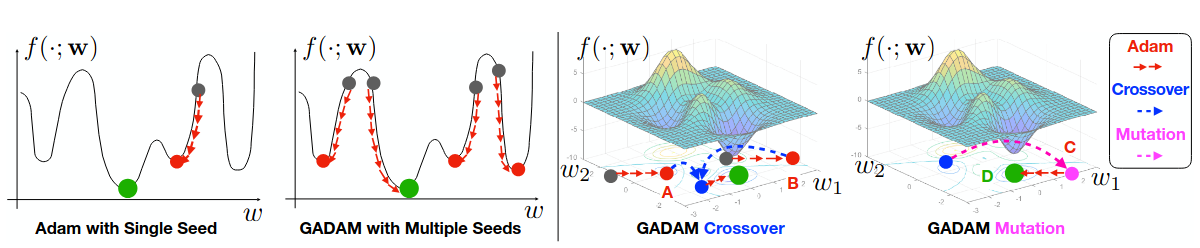
\includegraphics[width=1\textwidth]{img/GADAM.png}
    \caption{Funzionamento di GADAM. Immagine tratta da \cite{gadam2018}}
    \label{fig:GADAM}
\end{figure}
    
\chapter{Esperimenti}

\section{Introduzione}
In questo capitolo vengono presentati e analizzati in dettaglio i risultati degli esperimenti introdotti nel capitolo precedente, con l'obiettivo di valutare le prestazioni e l'efficacia dei diversi algoritmi di ottimizzazione applicati al training di reti neurali Multi-Layer Perceptron (MLP).
La sperimentazione è stata condotta seguendo una metodologia rigorosa e sistematica, al fine di garantire la comparabilità dei risultati e la validità delle conclusioni tratte. Gli esperimenti sono stati progettati per esplorare diverse dimensioni del problema di ottimizzazione: l'impatto della quantità di dati di training, l'influenza del numero di epoche, l'efficacia di approcci ibridi e i benefici della parallelizzazione.

\section{Allenamento con SGDM}
 L'allenamento della rete neurale MLP con SGDM, variando il numero di dati di training, ha generato i risultati mostrati in tabella. 
\begin{table}[htbp]
\centering
\begin{tabular}{|c|c|c|c|c|}
\hline
\textbf{Dati Training} & \textbf{Accuracy} & \textbf{Loss} & \textbf{Tempo (s)} & \textbf{Epoche} \\
\hline
1000 & 87.44\% & 0.436481 & 1.84 & 25 \\
\hline
5000 & 93.96\% & 0.236183 &  8.65 & 25 \\
\hline
10000 & 95.97\% & 0.153752 & 17.51 & 25 \\
\hline
15000 & 96.84\% &  0.115814 &28.69 & 25 \\
\hline
\end{tabular}
\label{tab:sgdm_results con 25 epoche}
\caption{Risultati allenamento SGDM con 25 epoche}
\end{table}

\newpage
Nella seguente tabella sono mostrati i risultati aumentando il numero di epoche a 100.
\begin{table}[htbp]
\centering
\begin{tabular}{|c|c|c|c|c|}
\hline
\textbf{Dati Training} & \textbf{Accuracy} & \textbf{Loss} & \textbf{Tempo (s)} & \textbf{Epoche} \\
\hline
1000 & 88.85\% & 0.581697 & 7.45 & 100 \\
\hline
5000 & 94.30 \% & 0.299773 &  36.93 & 100 \\
\hline
10000 & 96.14\% & 0.188318 & 75.97 & 100 \\
\hline
15000 & 96.94\% &  0.143579 & 112.85 & 100 \\
\hline
\end{tabular}
\label{tab:sgdm_results con 100 epoche}
\caption{Risultati allenamento SGDM con 100 epoche}
\end{table}

\section{Allenamento con GA}
    L'allenamento della rete neurale MLP con i GA, con vari metodi di crossover, utilizzando un numero di dati di training pari a 1000, ha generato i risultati mostrati in tabella.
    Come già detto precedentemente il numero di dati di training è stato scelto pari a 1000, in quanto l'allenamento con GA risulta essere molto più lento rispetto a SGDM, ADAM e le loro versioni ibride.
    Per questo motivo si è deciso di utilizzare un numero di dati di training più piccolo, per poter fare un confronto con gli altri metodi. Ovviamente questo comporta che bisogna confrontare i risultati
    ottenuti con GA con quelli ottenuti con SGDM con 1000 dati di training.
\begin{table}[htbp]
\centering
\begin{tabular}{|c|c|c|c|c|c|c|}
\hline
\textbf{Dati Train} & \textbf{Cross.} & \textbf{Accuracy} & \textbf{Loss} & \textbf{Tempo (h)} & \textbf{Gen.} & \textbf{Pop.} \\
\hline
1000 & Aritmetico & 66\% & 1.3410 & 2.5 & 250 & 100 \\
\hline
1000 & Blend & 74.90\% & 1.1595 & 2.5 & 250 & 100 \\
\hline
1000 & SBX & 58\% & 1.3022 & 2.5 & 250 & 100 \\
\hline
1000 & Adattivo & 70.20\% & 1.0636 & 2.5 & 250 & 100 \\
\hline
\end{tabular}
\label{tab:GA_results}
\caption{Risultati allenamento GA}
\end{table}
    Da questi esperimenti si può notare come il metodo di crossover più efficace sia stato il crossover blend, che ha portato ad una accuratezza del 74.90\% e una loss di 1.1595.
    C'è comunque da considerare, che seppur avendo tenuto lo stesso seed per tutti gli esperimenti, il GA è un algoritmo stocastico e quindi i risultati possono variare leggermente ad ogni esecuzione.
    Comunque si può notare come il GA non riesce a raggiungere le prestazioni di SGDM con 1000 dati di training, che ha portato ad una accuratezza dell'87.44\% e una loss di 0.436481.
    Questo è dovuto al fatto che il GA è un algoritmo di ottimizzazione globale, che cerca di esplorare tutto lo spazio delle soluzioni, ma non è molto efficace nel trovare soluzioni locali ottimali.
    Inoltre il tempo di allenamento è molto più lungo rispetto a SGDM, come si può notare dalla tabella, dove il tempo di allenamento con GA è di circa 2 ore, mentre con SGDM è di pochi secondi.
    Da ora in poi, per gli esperimenti con GA, si utilizzerà il crossover blend, essendo il metodo che ha prodotto i risultati migliori.
\section{Allenamento con GA parallelizzato}
    L'implementazione della parallelizzazione per l'allenamento della rete attraverso algoritmi genetici (GA) ha prodotto significativi miglioramenti in termini di efficienza computazionale, come evidenziato dai risultati presentati nella tabella seguente.
    La strategia di parallelizzazione adottata prevede l'utilizzo di otto processi simultanei, corrispondenti al numero di core logici del calcolatore utilizzato per la sperimentazione. Questa configurazione rappresenta il punto di equilibrio ottimale tra sfruttamento delle risorse hardware disponibili e prevenzione della contesa eccessiva per le risorse di sistema.
\begin{table}[htbp]
\centering
\begin{tabular}{|c|c|c|c|c|c|c|}
\hline
\textbf{Dati Train.} & \textbf{Cross.} & \textbf{Accuracy}& \textbf{Tempo (s)} & \textbf{Gen.} & \textbf{Pop.} & \textbf{Parallel.}\\
\hline
1000 & Blend & 66.68\%  & 7662.46 & 200 & 100 & No\\
\hline
1000 & Blend & 66.84\%  & 4637.13s & 200 & 100 & Si\\
\hline
\end{tabular}
\label{tab:GA_results}
\caption{Risultati allenamento GA}
\end{table}

    I dati sperimentali dimostrano chiaramente l'efficacia della parallelizzazione nell'ottimizzazione del processo di training. La versione parallelizzata dell'algoritmo ha conseguito una riduzione del tempo di esecuzione da 7662.46 secondi (circa 2.13 ore) a 4637.13 secondi (circa 1.29 ore), corrispondente a un miglioramento delle prestazioni del 39.5\% circa, mantenendo sostanzialmente invariata l'accuratezza del modello.
    L'efficacia della parallelizzazione è strettamente legata alle caratteristiche dell'architettura hardware utilizzata. L'impiego di otto processi paralleli, ha garantito un utilizzo ottimale delle risorse computazionali. È importante sottolineare che l'incremento del numero di processi oltre la capacità fisica del sistema tenderebbe a produrre un peggioramento delle prestazioni a causa della competizione per le risorse condivise.
    I risultati ottenuti suggeriscono un significativo potenziale di miglioramento delle prestazioni su architetture hardware più potenti. L'utilizzo di sistemi multi-core con un maggior numero di unità di elaborazione parallele potrebbe portare a riduzioni ancora più sostanziali dei tempi di training, sfruttando la natura intrinsecamente parallela degli algoritmi genetici.

\section{Allenamento con GASGDM}
    In questa sezione vengono presentati i miglioramenti ottenuti dall'utilizzo combinato di Algoritmo Genetico (GA) e Stochastic Gradient Descent with Momentum (SGDM), rispetto all'impiego del solo SGDM. 
    I test sono stati eseguiti su diverse partizioni del dataset, considerando set di training composti da 1.000, 5.000, 10.000 e 15.000 istanze. 
    I miglioramenti sono riportati nelle tabelle seguenti. È importante sottolineare che l'uso di GASGDM comporta un tempo di training maggiore rispetto al solo SGDM; tuttavia, questo è giustificato dal fatto che GASGDM è in grado di trovare soluzioni che SGDM non riuscirebbe a individuare nemmeno aumentando significativamente il numero di epoche.
    Per questi esperimenti sono stati scelti i seguenti parametri per GA e SGDM:
    \begin{compactitemize}
        \item \textbf{Numero di generazioni}: 10
        \item \textbf{Popolazione}: 10
        \item \textbf{Numero di cicli GASGDM}: 3
        \item \textbf{Epoche SGDM}: 10
    \end{compactitemize}


\begin{table}[htbp]
\centering
\begin{tabular}{|c|c|c|c|c|}
\hline
\textbf{Dati Train.} & \textbf{Metodo} & \textbf{Accuracy} & \textbf{Tempo (s)} & \textbf{Epoche SGDM} \\
\hline
1000 & SGDM & 88.80\% & 3.64 & 50 \\
\hline
1000 & GASGDM & 89.51\% & 79.23 & 10 \\
\hline
\end{tabular}
\caption{Risultati dell'allenamento con GASGDM su 1.000 istanze di training}
\label{tab:GASGDM_results_1000}
\end{table}

\begin{table}[htbp]
\centering
\begin{tabular}{|c|c|c|c|c|}
\hline
\textbf{Dati Train.} & \textbf{Metodo} & \textbf{Accuracy} & \textbf{Tempo (s)} & \textbf{Epoche SGDM} \\
\hline
5000 & SGDM & 94.33\% & 18.17 & 50 \\
\hline
5000 & GASGDM & 95.00\% & 174.52 & 10 \\
\hline
\end{tabular}
\caption{Risultati dell'allenamento con GASGDM su 5.000 istanze di training}
\label{tab:GASGDM_results_5000}
\end{table}

\begin{table}[htbp]
\centering
\begin{tabular}{|c|c|c|c|c|}
\hline
\textbf{Dati Train.} & \textbf{Metodo} & \textbf{Accuracy} & \textbf{Tempo (s)} & \textbf{Epoche SGDM} \\
\hline
10000 & SGDM & 96.11\% & 22.21 & 50 \\
\hline
10000 & GASGDM & 96.37\% & 315.38 & 10 \\
\hline
\end{tabular}
\caption{Risultati dell'allenamento con GASGDM su 10.000 istanze di training}
\label{tab:GASGDM_results_10000}
\end{table}


\begin{table}[H]
    \centering
    \begin{tabular}{|c|c|c|c|c|}
    \hline
    \textbf{Dati Train.} & \textbf{Metodo} & \textbf{Accuracy} & \textbf{Tempo (s)} & \textbf{Epoche SGDM} \\
    \hline
    15000 & SGDM & 96.90\% & 33.60 & 50 \\
    \hline
    15000 & GASGDM & 96.96\% & 442.14 & 10 \\
    \hline
    \end{tabular}
    \caption{Risultati dell'allenamento con GASGDM su 15.000 istanze di training}
    \label{tab:GASGDM_results_15000}
    \end{table}
    Per valutare la capacità di GASGDM di superare i minimi locali dello SGDM, è stato eseguito un esperimento incrementando il numero di epoche di SGDM a 300 e 500, mentre il numero di cicli GASGDM è stato aumentato a 6 e le epoche SGDM a 20.
\begin{table}[H]
    \centering
    \begin{tabular}{|c|c|c|c|c|}
    \hline
    \textbf{Dati Train.} & \textbf{Metodo} & \textbf{Accuracy} & \textbf{Tempo (s)} & \textbf{Epoche SGDM} \\
    \hline
    15000 & SGDM & 97.00\% & 465.55 & 300 \\
    \hline
    15000 & SGDM & 97.00\% & 771.12 & 500 \\
    \hline
    15000 & GASGDM & 97.06\% & 1484 & 20 \\
    \hline
    \end{tabular}
    \caption{Confronto tra SGDM e GASGDM su 15.000 istanze con epoche SGDM aumentate}
    \label{tab:GASGDM_results2_15000}
    \end{table}
    Dai risultati ottenuti emerge come l'efficacia dei metodi basati sul gradiente aumenti con l'incremento del numero di dati di training, consentendo di raggiungere buone soluzioni in tempi relativamente brevi. 
    Tuttavia, è importante sottolineare che GASGDM riesce a individuare soluzioni migliori rispetto al solo SGDM anche con un numero ridotto di epoche, dimostrando la sua capacità di superare minimi locali e ottimizzare in maniera più efficace.


\begin{figure}[htbp]
    \centering
    \begin{tikzpicture}
    \begin{axis}[
        width=13cm,
        height=7cm,
        xlabel={Numero dati di training},
        ylabel={Accuratezza (\%)},
        ymin=85, ymax=98,
        xtick={1000,5000,10000,15000},
        legend pos=south east,
        ymajorgrids=true,
        grid style=dashed
    ]
    
    % SGDM
    \addplot[
        color=green!60!black,
        mark=triangle*
    ] coordinates {
        (1000,88.80) (5000,94.33) (10000,96.11) (15000,96.80)
    };
    \addlegendentry{SGDM}
    
    % GASGDM
    \addplot[
        color=orange,
        mark=diamond*
    ] coordinates {
        (1000,89.51) (5000,95.00) (10000,96.37) (15000,96.96)
    };
    \addlegendentry{GASGDM}
    
    \end{axis}
    \end{tikzpicture}
    \caption{Accuratezza di SGDM vs GASGDM al variare della dimensione del dataset}
    \end{figure}
    
\section{Allenamento con GADAM}
    In questa sezione sono mostrati i miglioramenti ottenuti combinando GA e ADAM, che hanno permesso di trovare soluzioni migliori rispetto all’utilizzo del solo ADAM. I test sono stati fatti su 
    varie partizioni di dataset, in particolare è stato testato il comportamento su 1000, 5000, 10000 e 15000 istanze di training.
    I miglioramenti sono mostrati in tabella, ovviamente c'è da considerare il tempo maggiore per fare il training con GADAM, ciò è giustificato dal fatto che GADAM riesce a trovare soluzioni che altrimenti sarebbero impossibili da ottenere.
    Per fare questi esperimenti si è deciso di utilizzare i seguenti parametri per il GA e SGDM:
    \begin{compactitemize}
        \item \textbf{Numero di generazioni}: 10
        \item \textbf{Popolazione}: 5
        \item \textbf{Numero cicli GADAM}: variabile in base al numero di dati di training
        \item \textbf{Epoche ADAM}: 50
    \end{compactitemize}

\begin{table}[H]
\centering
\begin{tabular}{|c|c|c|c|c|c|}
\hline
\textbf{Dati Train.} & \textbf{Metodo} & \textbf{Accuracy}& \textbf{Tempo (s)} & \textbf{Epoche GADAM}\\
\hline
1000 & ADAM & 90.30\%  & 0.52 & 50 \\
\hline
1000 & GADAM &  90.67\%  & 77.13 & 50\\
\hline
\end{tabular}
\label{tab:GADAM_results_1000}
\caption{Risultati allenamento GADAM con 1000 istanze di training}
\end{table}


\begin{table}[htbp]
\centering
\begin{tabular}{|c|c|c|c|c|c|}
\hline
\textbf{Dati Train.} & \textbf{Metodo} & \textbf{Accuracy}& \textbf{Tempo (s)} & \textbf{Epoche GADAM}\\
\hline
5000 & ADAM & 95.20\%  & 25.80 & 50 \\
\hline
5000 & GADAM & 95.86\%  & 375.23  & 50\\
\hline
\end{tabular}
\label{tab:GADAM_results_5000}
\caption{Risultati allenamento GADAM con 5000 istanze di training}
\end{table}


\begin{table}[htbp]
\centering
\begin{tabular}{|c|c|c|c|c|c|}
\hline
\textbf{Dati Train.} & \textbf{Metodo} & \textbf{Accuracy}& \textbf{Tempo (s)} & \textbf{Epoche GADAM}\\
\hline
10000 & ADAM & 96.72\%  & 58.3 & 50 \\
\hline
10000 & GADAM &  97.07\%  & 750.45 & 50\\
\hline
\end{tabular}
\label{tab:GADAM_results_10000}
\caption{Risultati allenamento GADAM con 10000 istanze di training}
\end{table}

\begin{table}[htbp]
\centering
\begin{tabular}{|c|c|c|c|c|c|}
\hline
\textbf{Dati Train.} & \textbf{Metodo} & \textbf{Accuracy}& \textbf{Tempo (s)} & \textbf{Epoche GADAM} \\
\hline
15000 & ADAM & 97.52\%  & 69.92 & 50 \\
\hline
15000 & GADAM & 97.62\%  & 1086.11 & 50\\
\hline
\end{tabular}
\label{tab:GADAM_results_15000}
\caption{Risultati allenamento GADAM con 15000 istanze di training}
\end{table}
    Ora per dimostare che Adam è bloccato in un minimo locale vediamo come si comporta aumentando il numero di epoche a 100 e 200, mentre in GADAM abbiamo aumentato la popolazione a 10 individui.
\begin{table}[H]
    \centering
    \begin{tabular}{|c|c|c|c|c|c|}
    \hline
    \textbf{Dati Train.} & \textbf{Metodo} & \textbf{Accuracy}& \textbf{Tempo (s)} & \textbf{Epoche GADAM} \\
    \hline
    15000 & ADAM & 97.42\%  & 146.41 & 100 \\
    \hline
    15000 & ADAM & 97.33\%  & 326.32 & 200\\
    \hline
    15000 & GADAM & 97.64\%  & 1153.79  & 50\\
    \hline
    \end{tabular}
    \label{tab:GADAM_results_15000_update}
    \caption{Risultati allenamento GADAM con 15000 istanze di training ma più epoche}
    \end{table}

    Dai risultati ottenuti si può notare come GADAM sia riuscito a trovare soluzioni migliori rispetto al solo ADAM.
    Ovviamente il tempo di allenamento è maggiore, ma questo è giustificato dal fatto che GADAM riesce a trovare soluzioni che ADAM non riuscirebbe a trovare nemmeno aumentando notevolmente le epoche.


\begin{figure}[htbp]
    \centering
    \begin{tikzpicture}
    \begin{axis}[
        width=13cm,
        height=7cm,
        xlabel={Numero dati di training},
        ylabel={Accuratezza (\%)},
        ymin=85, ymax=98,
        xtick={1000,5000,10000,15000},
        legend pos=south east,
        ymajorgrids=true,
        grid style=dashed
    ]
    
    % ADAM
    \addplot[
        color=blue,
        mark=square
    ] coordinates {
        (1000,90.30) (5000,95.2) (10000,96.72) (15000,97.52)
    };
    \addlegendentry{ADAM}
    
    % GADAM
    \addplot[
        color=red,
        mark=*
    ] coordinates {
        (1000,90.67) (5000,95.86) (10000,97.07) (15000,97.63)
    };
    \addlegendentry{GADAM}
    
    \end{axis}
    \end{tikzpicture}
    \caption{Accuratezza di ADAM vs GADAM al variare della dimensione del dataset}
    \end{figure}
    
\newgeometry{top=1.5cm, bottom=1.5cm, left=3cm, right=3cm} 
\chapter{Conclusioni}
\begin{flushleft}
    La presente tesi ha fornito una panoramica dettagliata sull'applicazione degli algoritmi genetici per l'addestramento delle reti neurali. Sono stati analizzati approfonditamente i principi teorici del machine learning, le architetture delle reti neurali e i meccanismi degli algoritmi evolutivi, presentando inoltre gli strumenti software utilizzati per lo sviluppo del progetto e la struttura metodologica del lavoro svolto.
    L'obiettivo principale di questo lavoro non è stato quello di sviluppare una soluzione  superiore alle tecniche esistenti, ma piuttosto di esplorare e validare un approccio alternativo all'addestramento delle reti neurali. La ricerca si è concentrata nel dimostrare come gli algoritmi genetici possano essere  utilizzati per l'ottimizzazione dei pesi delle reti neurali, offrendo un metodo alternativo rispetto alle consolidate tecniche di backpropagation tradizionali.\\
    Per garantire un confronto metodologicamente coerente tra i diversi approcci, è stata  utilizzata la funzione di cross-entropy come metrica di valutazione, pur non sfruttando completamente le potenzialità degli algoritmi genetici. Va sottolineato infatti che la caratteristica peculiare e distintiva di questi algoritmi è la loro capacità di operare efficacemente senza richiedere la differenziabilità della funzione obiettivo, proprietà particolarmente vantaggiosa in numerosi contesti applicativi come il reinforcement learning, dove questa caratteristica matematica non è sempre disponibile o facilmente implementabile.\\
    I risultati sperimentali ottenuti hanno evidenziato alcuni aspetti interessanti degli algoritmi genetici nell'addestramento delle reti neurali, sebbene nel caso studio specifico analizzato non siano riusciti a raggiungere le prestazioni del metodo tradizionale di riferimento. Tuttavia, è emerso come la combinazione di entrambi gli approcci metodologici possa potenzialmente portare a risultati più promettenti rispetto all'utilizzo esclusivo di una singola tecnica.
\end{flushleft}

%---------------------- Ringraziamenti -----------------------%
\newpage
\chapter*{Ringraziamenti}
\thispagestyle{empty} % Rimuove intestazioni e numeri di pagina
\addcontentsline{toc}{chapter}{Ringraziamenti} % Aggiunge ai segnalibri e all'indice

Il mio primo e più sentito ringraziamento va al professore Calderara che è da subito stato molto disponibile nel seguirmi durante la realizzazione della tesi, e ringrazio ancora di più per aver accolto la mia idea di lavorare con gli algoritmi genetici e reti neurali, argomenti non affrontati durante la triennale, dandomi la possibilità di spingermi oltre.\\

Un ringraziamento speciale va alla mia famiglia, che è stata il mio punto fermo durante tutto il percorso universitario. Grazie per avermi sempre sostenuto, incoraggiato e spronato a dare il massimo, anche nei momenti più difficili. Senza il vostro affetto, la vostra pazienza e la fiducia che avete riposto in me, non sarei mai riuscito a raggiungere questo traguardo.\\

Non posso non ringraziare i miei colleghi con cui ho trascorso tanti momenti di studio e confronto, rendendo il percorso universitario più piacevole e stimolante.\\ In particolare vorrei ringraziare Giulia e Christian per essere stati sempre disponibili al confronto e alla discussione e per esserci stati fino all'ultimo momento, rendendo questo duro percorso molto più leggero.\\ Ringrazio anche il trio con cui ho passato i momenti più divertenti durante questo percorso, ovvero Rocco, Vincenzo e Marcello. Anche se nell'ultimo periodo eravate poco presenti a lezione, ho ricordi indelebili che porterò sempre con me.\\

Un grande ringraziamento va ai miei amici di sempre, in particolare Giacomo, Alessandro ed Emilia, che mi hanno sempre sostenuto, seppur da lontano, e fatto compagnia durante questi intensi anni.\\

A tutti voi, un grande grazie di cuore.
\newpage


%---------------------- Bibliografia -------------------------%
\begin{thebibliography}{9}

  \bibitem{Github_for_code}
  Repository GitHub del progetto. Available at \url{https://github.com/Ro253ck/Bachelor_thesis.git}
  \bibitem{gadam2018}
  Jiawei Zhang and Fisher B. Gouza.
  \textit{GADAM: Genetic-Evolutionary ADAM for Deep Neural Network Optimization}. 
  arXiv preprint arXiv:1805.07500, 2018.
  Available at \url{https://doi.org/10.48550/arXiv.1805.07500}.
  
  \bibitem{kingma2017}
  Diederik P. Kingma and Jimmy Ba.
  \textit{Adam: A Method for Stochastic Optimization}.
  arXiv preprint arXiv:1412.6980, 2017.
  Available at \url{https://arxiv.org/abs/1412.6980}.
  
  \bibitem{Introduction_to_Machine_Learning_book}
  Ethem Alpaydin.
  \textit{Introduction to Machine Learning, second edition.}

  \bibitem{Introduction to Evolutionary Computing. Springer.}
  A.E. Eiben and J.E. Smith.
  \textit{Introduction to Evolutionary Computing. Springer.}

  \bibitem{Double_Descent_Image}
  Dkarkada.
  \textit{Double descent} [Image]. Wikimedia Commons, 2 May 2023. 
  Available at \url{https://commons.wikimedia.org/wiki/File:Double_descent.png}.

  \bibitem{Bias_Variance_Image}
  Bigbossfarin.
  \textit{Bias and variance contributing to total error} [Image]. Wikimedia Commons, 15 May 2021. 
  Available at \url{https://commons.wikimedia.org/wiki/File:Bias_and_variance_contributing_to_total_error.svg}.

  \bibitem{Sigmoid_Function_Image}
  MartinThoma.
  \textit{Sigmoid function} [Image]. Wikimedia Commons, 25 May 2014. 
  Available at \url{https://commons.wikimedia.org/wiki/File:Sigmoid-function-2.svg}.

  \bibitem{MNIST_Examples_Image}
  Josef Steppan.
  \textit{A few samples from the MNIST test dataset} [Image]. Wikimedia Commons, 14 December 2017. 
  Available at \url{https://commons.wikimedia.org/wiki/File:MnistExamples.png}.

  \bibitem{GA_Image}
  OKpedia.
  \textit{Algoritmo Genetico} [Image]. OKpedia, 14 December 2014. 
  Available at: \url{https://www.okpedia.it/algoritmo_genetico}.

\end{thebibliography}
  


\end{document}
